\documentclass{article}
\usepackage{fancyhdr}
\usepackage{ctex}
\usepackage{listings}
\usepackage{graphicx}
\usepackage[a4paper, body={18cm,22cm}]{geometry}
\usepackage{amsmath,amssymb,amstext,wasysym,enumerate,graphicx}
\usepackage{float,abstract,booktabs,indentfirst,amsmath}
\usepackage{array}
\usepackage{booktabs}
\usepackage{multirow}
\usepackage{url}
\usepackage{diagbox}
\usepackage{hyperref}
\usepackage{listings}
\renewcommand\arraystretch{1.4}
\usepackage{indentfirst}
\setlength{\parindent}{2em}
\usepackage{enumitem}
\usepackage{accsupp}
\setmonofont{Consolas}
\usepackage{listings}
\usepackage{xcolor}
\usepackage{makecell}
\setCJKmonofont{黑体}
\newcommand\emptyaccsupp[1]{\BeginAccSupp{ActualText={}}#1\EndAccSupp{}}
\newcommand\SQL{\texttt{SQL}}
\renewcommand\tt{\texttt}
\lstset{
    % language = C,
    showstringspaces=false,
    xleftmargin = 3em,xrightmargin = 3em, aboveskip = 1em,
	backgroundcolor = \color{white}, % 背景色
	basicstyle = \small\ttfamily, % 基本样式 + 小号字体
	rulesepcolor= \color{gray}, % 代码块边框颜色
	breaklines = true, % 代码过长则换行
	numbers = left, % 行号在左侧显示
	numberstyle=\emptyaccsupp,
    numbersep = 14pt, 
    keywordstyle=\color{purple}\bfseries, % 关键字颜色
    commentstyle =\color{red!50!green!50!blue!60}, % 注释颜色
    stringstyle = \color{red}, % 字符串颜色
    morekeywords={ASSERT, int64_t, uint32_t},
	% frame = shadowbox, % 用(带影子效果)方框框住代码块
	frame = single, % 用(带影子效果)方框框住代码块
	showspaces = false, % 不显示空格
	columns = fixed, % 字间距固定
  framesep=1em
} 
\lstset{
    sensitive=true,
    moreemph={ASSERT, NULL}, emphstyle=\color{red}\bfseries,
    moreemph=[2]{int64_t, uint32_t, tid_t, uint8_t, int16_t, uint16_t, int32_t, size_t}, emphstyle=[2]\color{purple}\bfseries,
    showspaces = false, % 不显示空格
    }
%--------------------页眉--------------------%
\pagestyle{fancy}
\fancyhead[L]{}
\fancyhead[R]{}
\fancyhead[C]{《数据库系统及应用实践》课程实验报告}
\fancyfoot[C]{-\thepage-}
\renewcommand{\headrulewidth}{1.5pt}
%--------------------标题--------------------%
\begin{document}
\begin{center}
  \LARGE{{\textbf{\heiti 《数据库系统及应用实践》课程实验报告}}}

  \vspace{0.5em}

  \large 实验3:函数,存储过程与触发器
  \begin{table}[H]
    \centering
    \begin{tabular}{p{2cm}p{2cm}<{\centering}p{0.4cm}p{2cm}p{3cm}<{\centering}p{0.4cm}p{2cm}p{3cm}<{\centering}}
      姓\qquad 名: & 李鹏达 & \quad & 学\qquad 号: & 10225101460 & \quad & 完成日期: & 2024年4月18日 \\ \cline{2-2} \cline{5-5} \cline{8-8}
    \end{tabular}
  \end{table}
\end{center}
% \rule{\textwidth}{1pt}
%--------------------正文--------------------%
\section{实验目标}
\begin{enumerate}[noitemsep]
  \item 学习 \texttt{MySQL} 数据库管理系统中用户自定义函数、存储过程和触发器的基本概念和语法;
  \item 能够根据要求编写正确的自定义函数、存储过程和触发器;
  \item 学习 \texttt{MySQL} 数据库管理系统中的递归查询和窗口函数等进阶查询功能;
\end{enumerate}

\section{实验过程记录}

\subsection{使用命令行客户端创建函数与存储过程}

\begin{enumerate}
  \item 打开命令行,启动一个 \texttt{MySQL} 容器示例;

        \begin{lstlisting}[language=bash]
sudo docker start dbcourse
\end{lstlisting}

        \begin{figure}[H]
          \centering
          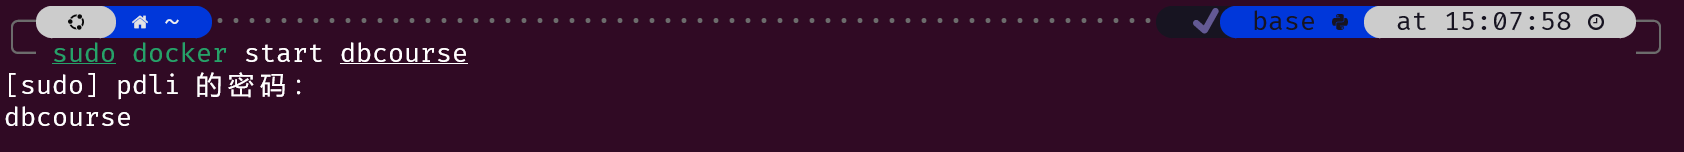
\includegraphics[width=0.9\textwidth]{img/1.png}
          \caption{启动 \texttt{MySQL} 容器示例}
        \end{figure}

  \item 在容器内启动一个 \texttt{bash} 终端,使用 \texttt{mysql} 命令登录到 \texttt{MySQL} 数据库;

        \begin{lstlisting}[language=bash]
sudo docker exec -it dbcourse bash
mysql -u root -p -D dbcourse
\end{lstlisting}

        \begin{figure}[H]
          \centering
          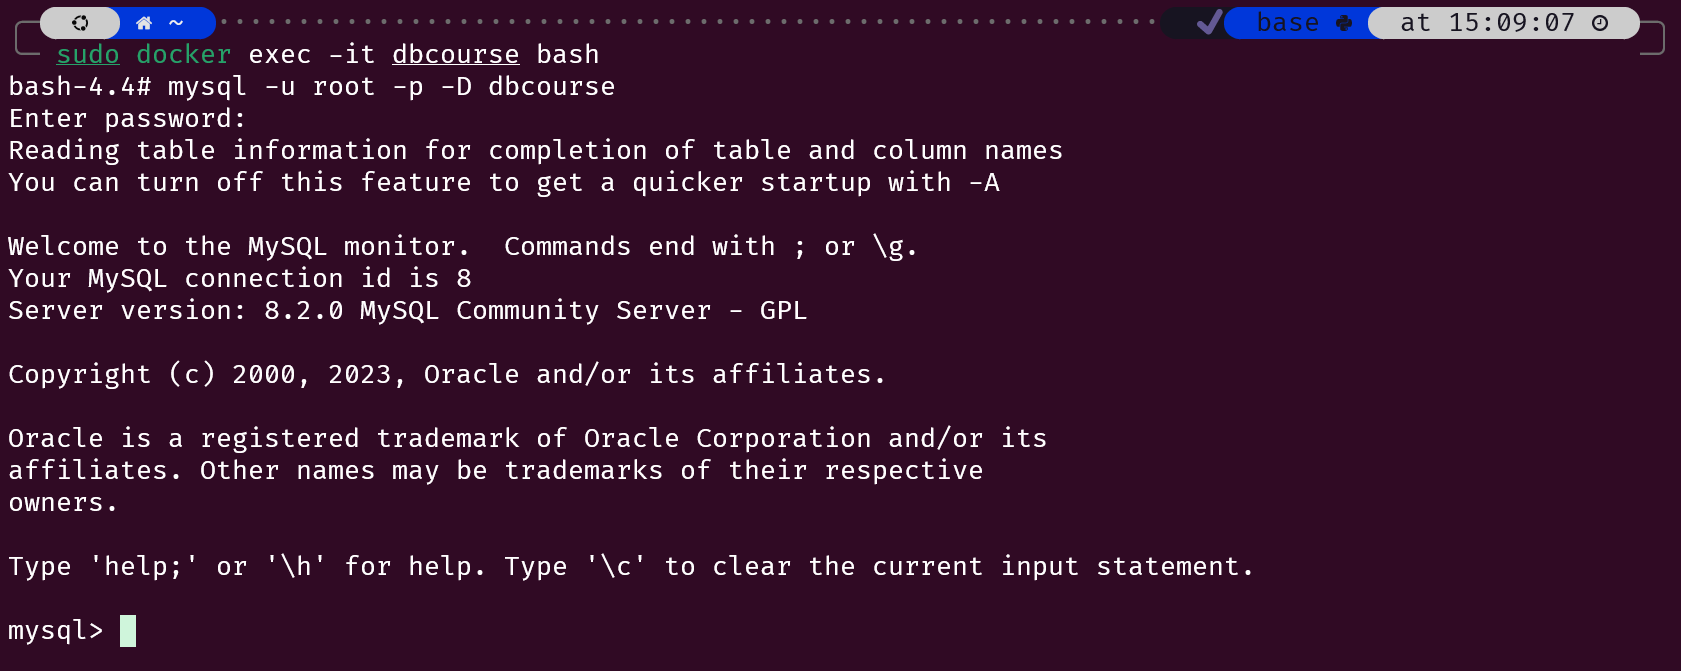
\includegraphics[width=0.9\textwidth]{img/2.png}
          \caption{登录到 \texttt{MySQL} 数据库}
        \end{figure}

  \item 参照教材199页Figure 5.6,创建一个名为\texttt{dept\_count}的用户自定义函数,用于统计指定院系的教师数量(返回一个值);

        \begin{lstlisting}[language=sql]
SET GLOBAL `log_bin_trust_function_creators` = 1;
DELIMITER $$
CREATE FUNCTION `dept_count`(`dept_name` VARCHAR(20)) RETURNS INT
BEGIN
    DECLARE `count` INT;
    SELECT COUNT(*) INTO `count` FROM `instructor` 
    WHERE `dept_name` = `instructor`.`dept_name`;
    RETURN `count`;
END$$
DELIMITER ;
\end{lstlisting}

        \begin{figure}[H]
          \centering
          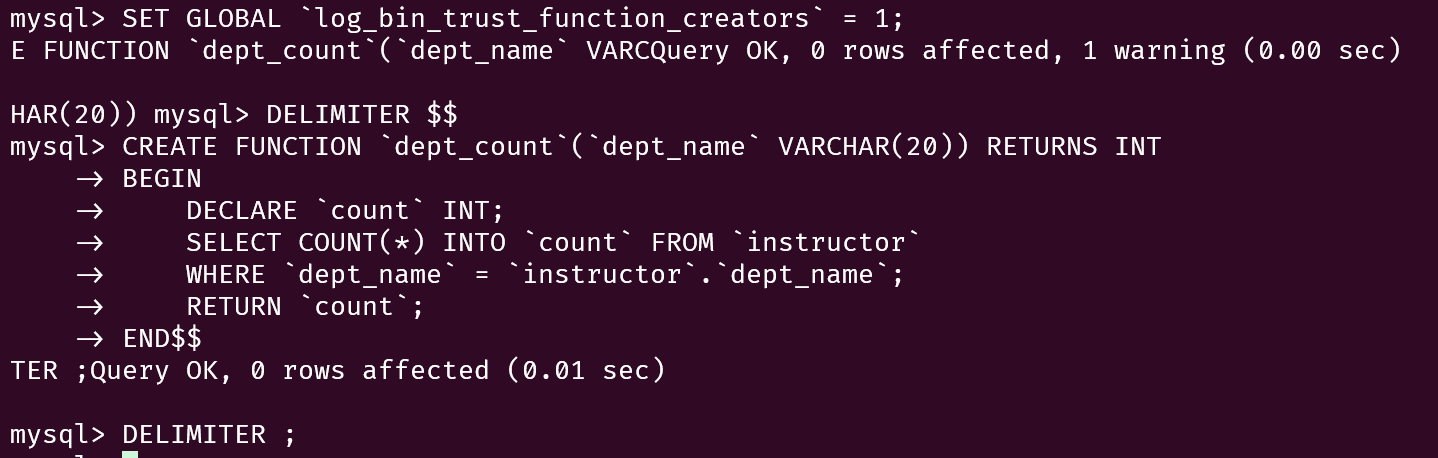
\includegraphics[width=0.9\textwidth]{img/3.png}
          \caption{创建自定义函数}
        \end{figure}

  \item 在SQL语句中调用自定义函数\texttt{dept\_count},查询计算机科学系(Comp. Sci.)和电子工程系(Elec. Eng.)的教师数量;

        \begin{lstlisting}[language=sql]
SELECT `dept_count`('Comp. Sci.'), `dept_count`('Elec. Eng.');
\end{lstlisting}

        \begin{figure}[H]
          \centering
          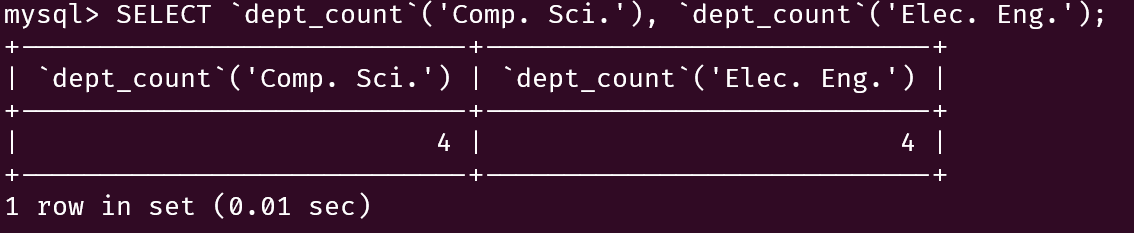
\includegraphics[width=0.9\textwidth]{img/4.png}
          \caption{运行自定义函数}
        \end{figure}

  \item 编写\SQL 语句,使用自定义函数\texttt{dept\_count}查询教师数量超过4人的院系名称和预算;

        \begin{lstlisting}[language=sql]
SELECT `dept_name`, `budget` 
FROM `department` 
WHERE `dept_count`(`dept_name`) > 4;
\end{lstlisting}

        \begin{figure}[H]
          \centering
          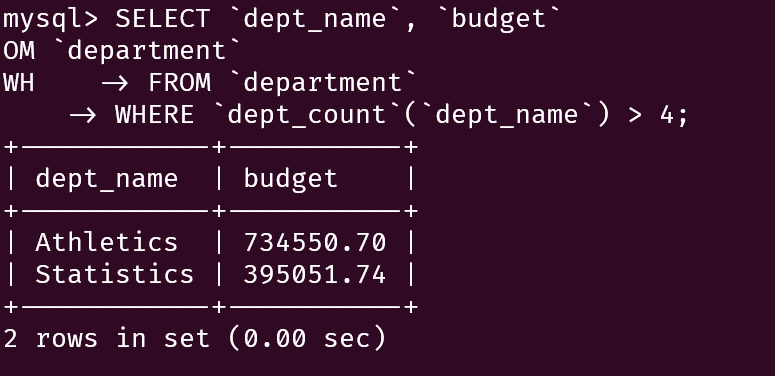
\includegraphics[width=0.9\textwidth]{img/5.png}
          \caption{查询结果}
        \end{figure}

  \item 将自定义函数\tt{dept\_count}改写成一个名为\tt{dept\_count\_proc}的存储过程;

        \begin{lstlisting}[language=sql]
DELIMITER $$
CREATE PROCEDURE `dept_count_proc`(
  IN `dept_name` VARCHAR(20),
  OUT `count` INT
)
BEGIN
  SELECT COUNT(*) INTO `count` FROM `instructor` 
  WHERE `dept_name` = `instructor`.`dept_name`;
END$$
DELIMITER ;
\end{lstlisting}

        \begin{figure}[H]
          \centering
          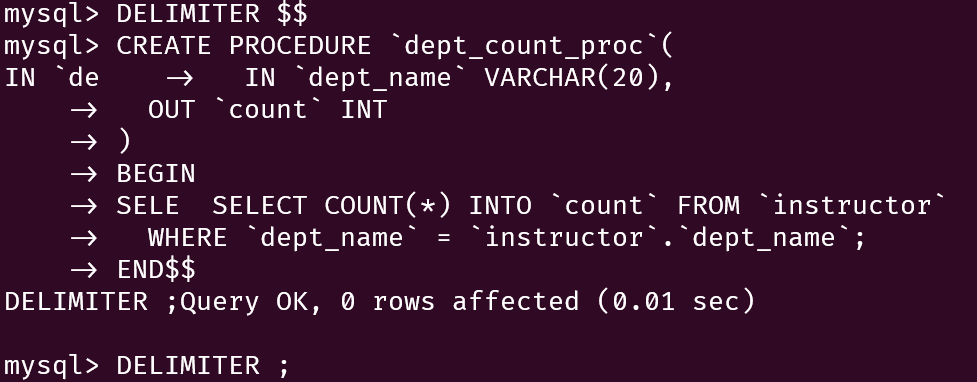
\includegraphics[width=0.6\textwidth]{img/6.png}
          \caption{创建存储过程}
        \end{figure}

  \item 通过\tt{call}语句调用存储过程\tt{dept\_count\_proc},查询生物系(Biology)和数学系(Math)的教师数量;

        \begin{lstlisting}[language=sql]
CALL `dept_count_proc`('Biology', @bio_count);
CALL `dept_count_proc`('Math', @math_count);
SELECT @bio_count, @math_count;
\end{lstlisting}

        \begin{figure}[H]
          \centering
          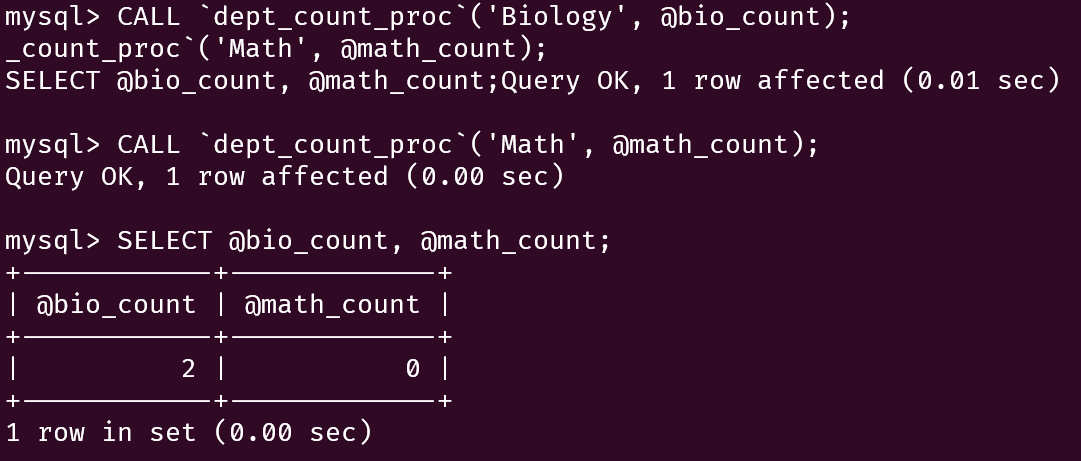
\includegraphics[width=0.7\textwidth]{img/7.png}
          \caption{调用存储过程}
        \end{figure}

  \item 删除自定义函数\tt{dept\_count}和存储过程\tt{dept\_count\_proc};

        \begin{lstlisting}[language=sql]
DROP FUNCTION `dept_count`;
DROP PROCEDURE `dept_count_proc`;
\end{lstlisting}

        \begin{figure}[H]
          \centering
          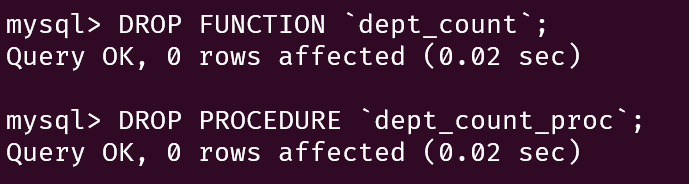
\includegraphics[width=0.5\textwidth]{img/8.png}
          \caption{删除自定义函数和存储过程}
        \end{figure}

\end{enumerate}

\subsection{使用\tt{Navicat}创建函数与存储过程}

\begin{enumerate}
  \item 启动\texttt{Navicat}应用,按以下步骤打开“函数向导”对话框
        \begin{enumerate}
          \item 连接到\tt{dbcourse}数据库;
          \item 单击工具栏中的“函数”按钮;
          \item 单击“新建函数”按钮,打开“函数向导对话框”;
        \end{enumerate}

        \begin{figure}[H]
          \centering
          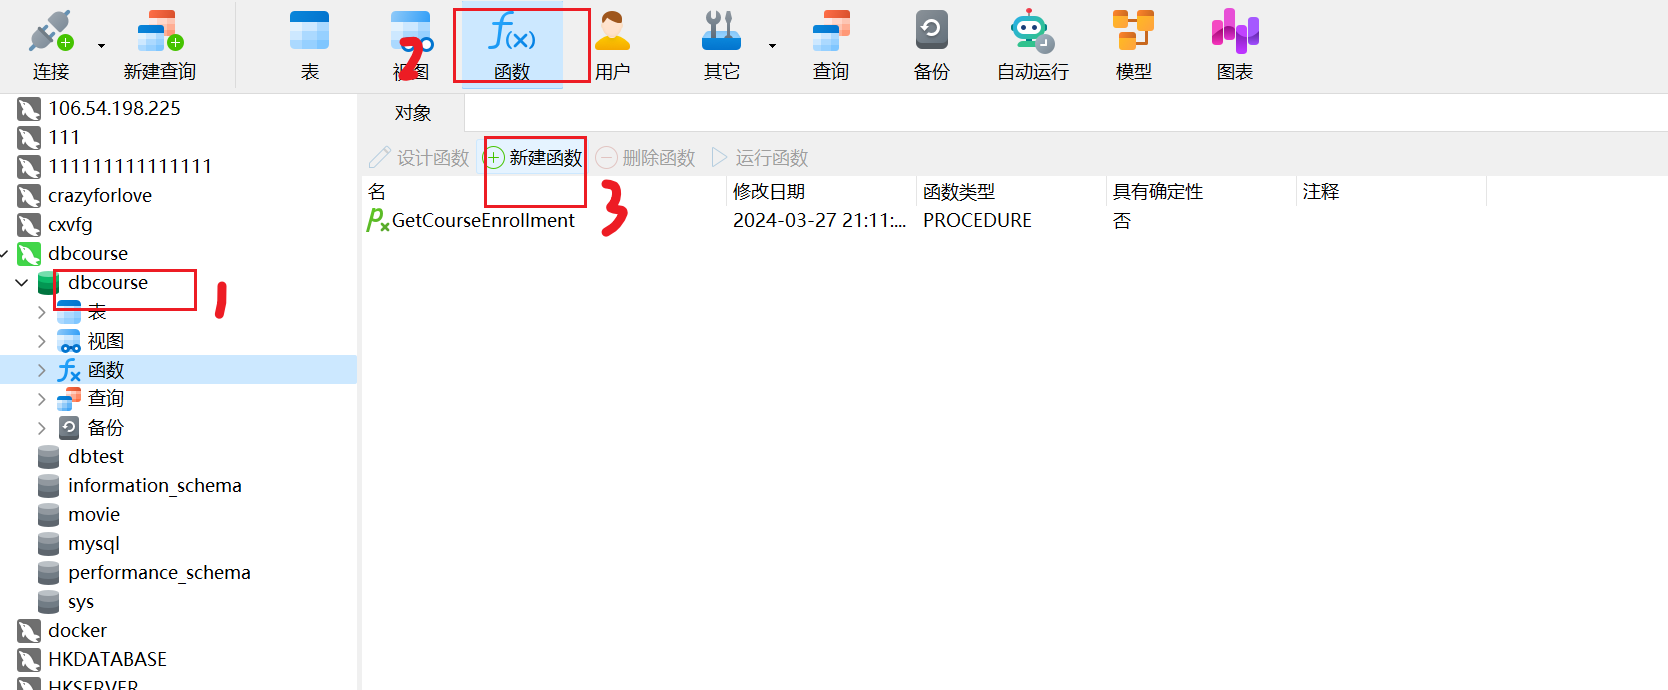
\includegraphics[width=0.9\textwidth]{img/9.png}
          \caption{根据流程创建函数}
        \end{figure}

  \item 参照教材203页Figure 5.8,创建一个名为\tt{register\_student}的存储过程,用于为学生注册课程;

        \begin{figure}[H]
          \centering
          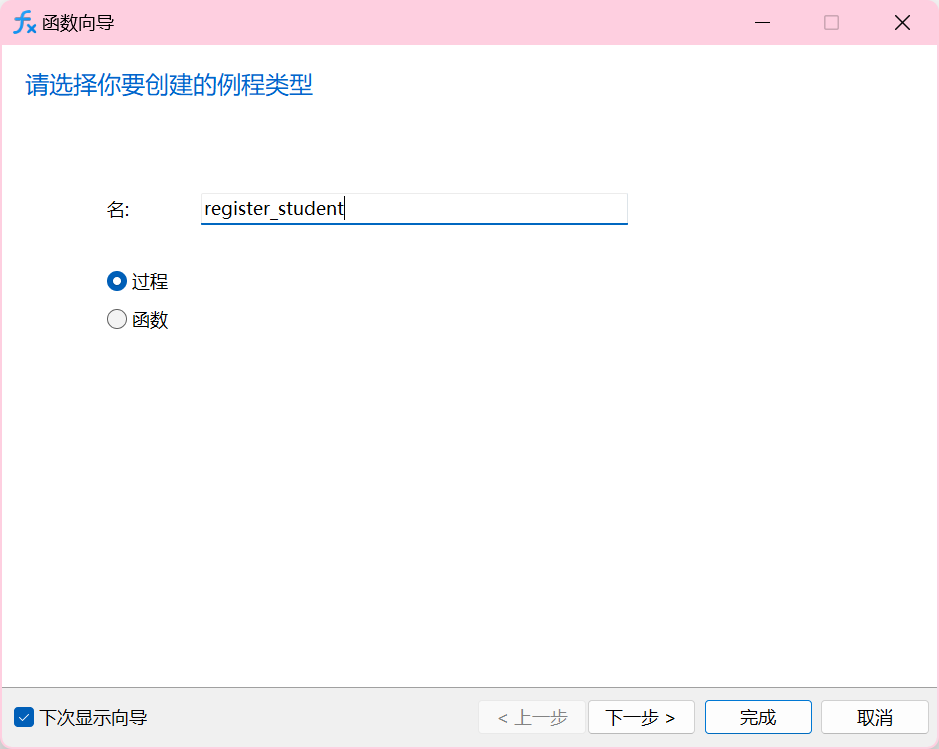
\includegraphics[width=0.6\textwidth]{img/10.png}
          \caption{创建存储过程}
        \end{figure}

        \begin{figure}[H]
          \centering
          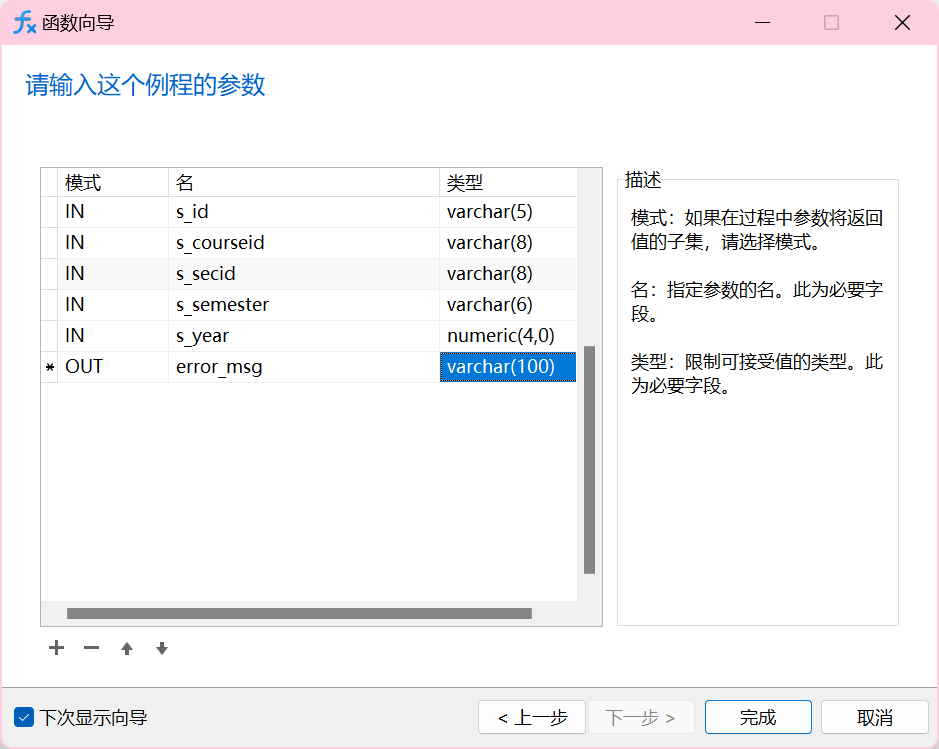
\includegraphics[width=0.6\textwidth]{img/11.png}
          \caption{设置参数}
        \end{figure}

        \begin{figure}[H]
          \centering
          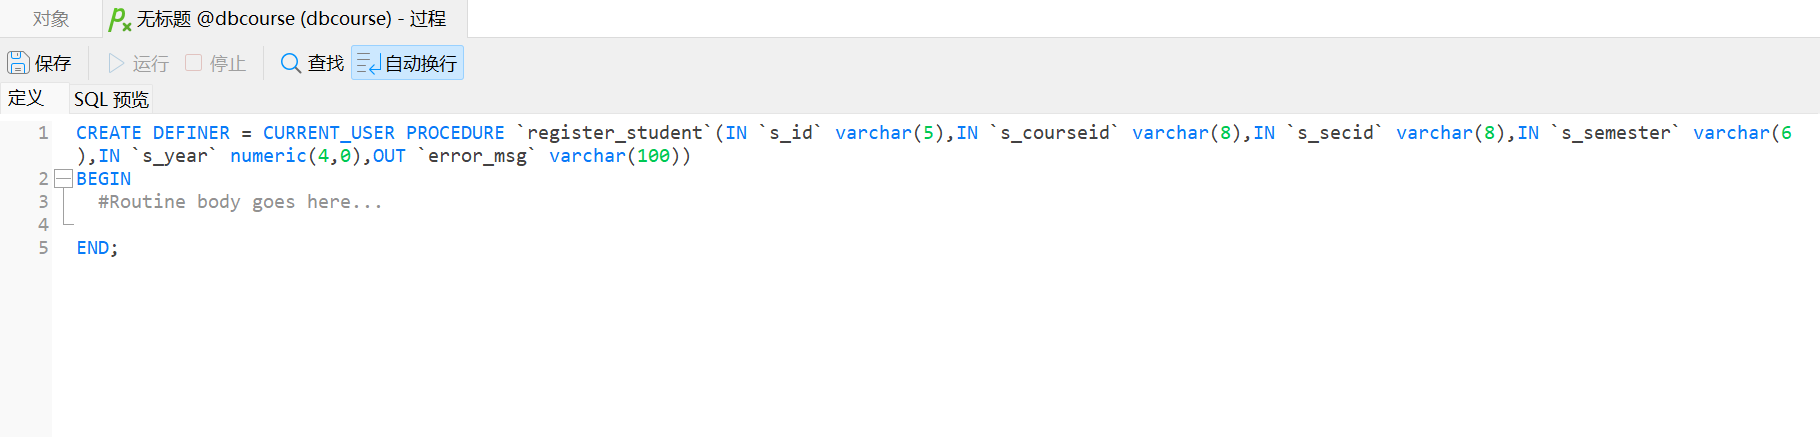
\includegraphics[width=0.9\textwidth]{img/12.png}
          \caption{编写代码}
        \end{figure}

        \begin{lstlisting}[language=sql]
CREATE DEFINER = CURRENT_USER PROCEDURE `register_student`(
  IN `s_id` varchar(5),
  IN `s_courseid` varchar(8),
  IN `s_secid` varchar(8),
  IN `s_semester` varchar(6),
  IN `s_year` numeric(4, 0),
  OUT `error_msg` varchar(100)
)
BEGIN
  -- #Routine body goes here...
  DECLARE `current_enrollment` INT;
  DECLARE `limit_capacity` INT;
  SELECT COUNT(*) INTO `current_enrollment` FROM `takes`
  WHERE `course_id` = `s_courseid` AND `sec_id` = `s_secid`
    AND `semester` = `s_semester` AND `year` = `s_year`;
  SELECT `capacity` INTO `limit_capacity` FROM `classroom`
  NATURAL JOIN `section`
  WHERE `course_id` = `s_courseid` AND `sec_id` = `s_secid`
    AND `semester` = `s_semester` AND `year` = `s_year`;
  IF (`current_enrollment` < `limit_capacity`) THEN 
  BEGIN
    INSERT INTO `takes` 
    VALUES (`s_id`, `s_courseid`, `s_secid`, `s_semester`, `s_year`, NULL);
    SET `error_msg` = 'Successful!';
  END;
  ELSE
    SET `error_msg` = CONCAT('Enrollment limit reached for course ', `s_courseid`, ' section ', `s_secid`);
  END IF;
END;
\end{lstlisting}

        \begin{figure}[H]
          \centering
          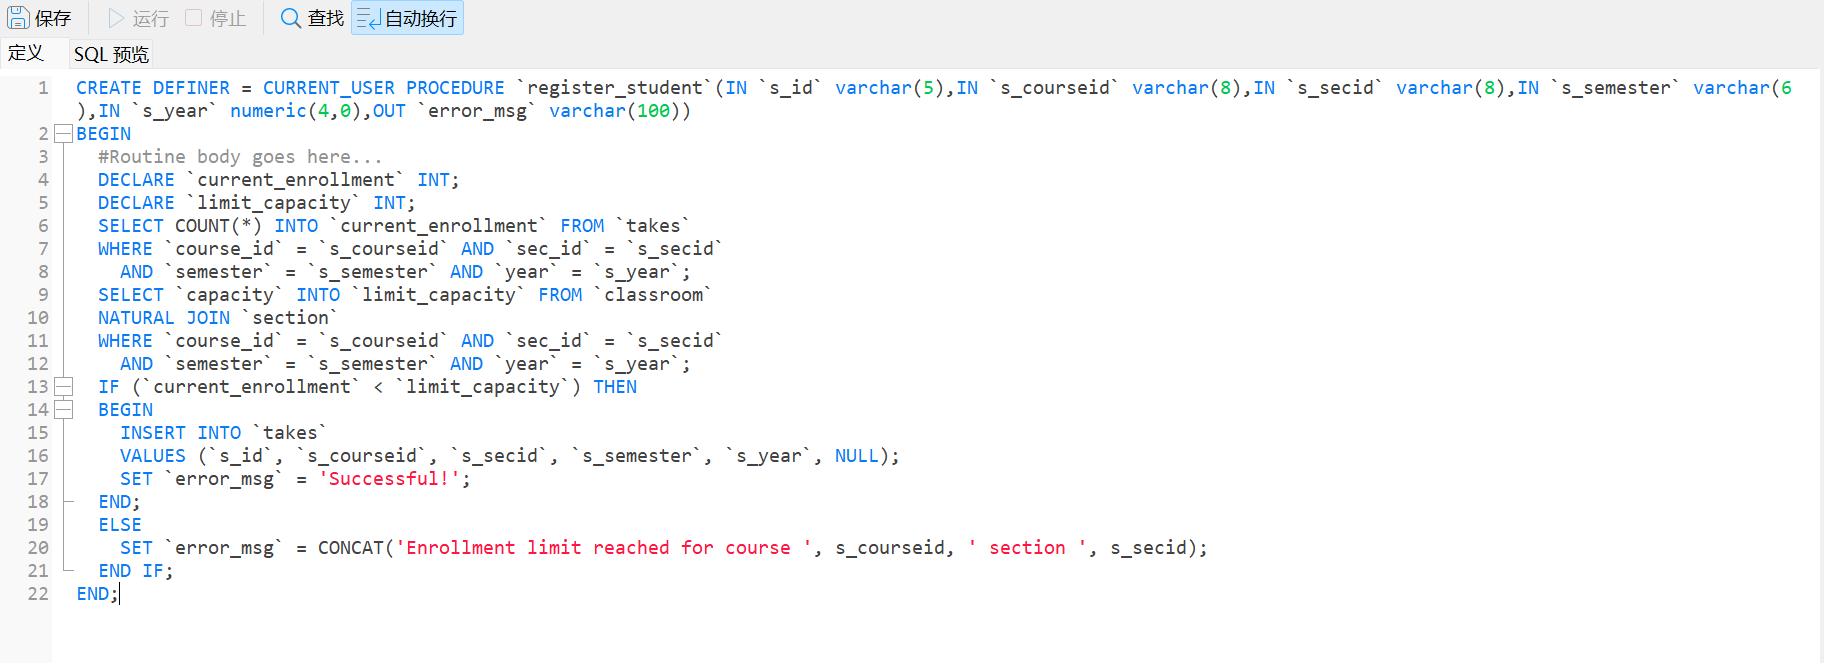
\includegraphics[width=0.9\textwidth]{img/13.png}
          \caption{保存存储过程}
        \end{figure}

  \item 在\tt{Navicat}的查询窗口中通过\tt{call}语句调用存储过程\tt{register\_student},为学号10481的同学注册2009年秋季学期开设的105课程和2010年秋季学期开设的476课程;

        \begin{lstlisting}[language=sql]
CALL `register_student`('10481', '105', '1', 'Fall', 2009, @msg1);
CALL `register_student`('10481', '476', '1', 'Fall', 2010, @msg2);
SELECT @msg1, @msg2;
\end{lstlisting}

        结果为:

        \begin{figure}[H]
          \centering
          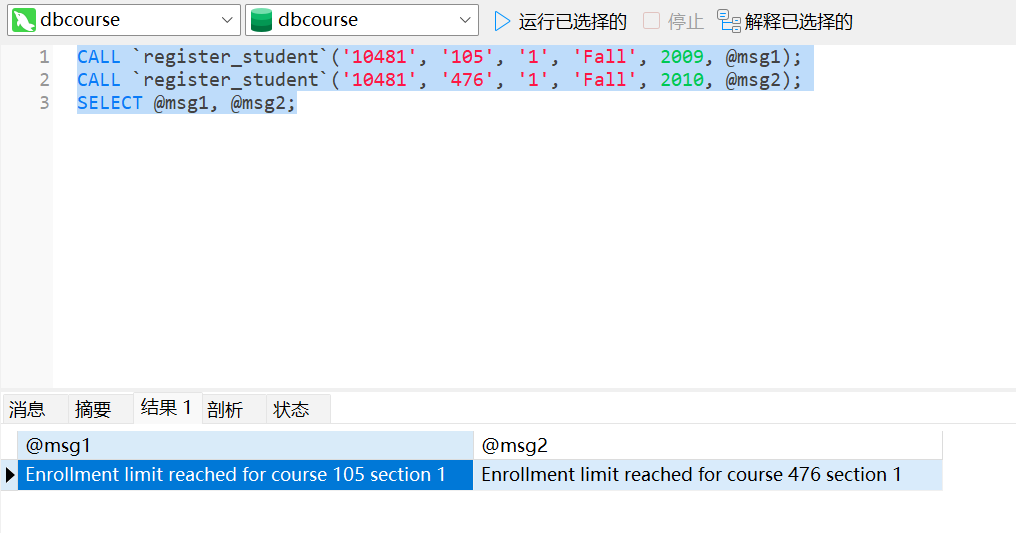
\includegraphics[width=0.9\textwidth]{img/14.png}
          \caption{调用存储过程}
        \end{figure}

  \item 显然,教材203页Figure 5.8中的处理逻辑并不完善,没有考虑不存在指定学号的学生和该学生已经注册了该门课程等情况,这就可能会导致存储过程异常退出。请对存储过程\tt{register\_student}的处理逻辑进行完善,确保其能正确处理各种情况并返回正确的结果。

        \begin{lstlisting}[language=sql]
DROP PROCEDURE `register_student`;
DELIMITER $$
CREATE DEFINER = CURRENT_USER PROCEDURE `register_student`(
  IN `s_id` varchar(5),
  IN `s_courseid` varchar(8),
  IN `s_secid` varchar(8),
  IN `s_semester` varchar(6),
  IN `s_year` numeric(4, 0),
  OUT `error_msg` varchar(100)
)
BEGIN
  -- #Routine body goes here...
  DECLARE `current_enrollment` INT;
  DECLARE `limit_capacity` INT;
  DECLARE `student_exist` INT;
  DECLARE `course_exist` INT;
  DECLARE `student_registered` INT;
  SELECT COUNT(*) INTO `student_exist` FROM `student`
  WHERE `ID` = `s_id`;
  SELECT COUNT(*) INTO `course_exist` FROM `section`
  WHERE `course_id` = `s_courseid` AND `sec_id` = `s_secid`
    AND `semester` = `s_semester` AND `year` = `s_year`;
  SELECT COUNT(*) INTO `student_registered` FROM `takes`
  WHERE `ID` = `s_id` AND `course_id` = `s_courseid` AND `sec_id` = `s_secid`
    AND `semester` = `s_semester` AND `year` = `s_year`;
  IF (`student_exist` = 0) THEN
    SET `error_msg` = 'Student does not exist!';
  ELSEIF (`course_exist` = 0) THEN
    SET `error_msg` = 'Course does not exist!';
  ELSEIF (`student_registered` > 0) THEN
    SET `error_msg` = 'Student has already registered this course!';
  ELSE
    SELECT COUNT(*) INTO `current_enrollment` FROM `takes`
    WHERE `course_id` = `s_courseid` AND `sec_id` = `s_secid`
      AND `semester` = `s_semester` AND `year` = `s_year`;
    SELECT `capacity` INTO `limit_capacity` FROM `classroom`
    NATURAL JOIN `section`
    WHERE `course_id` = `s_courseid` AND `sec_id` = `s_secid`
      AND `semester` = `s_semester` AND `year` = `s_year`;
    IF (`current_enrollment` < `limit_capacity`) THEN
    BEGIN
      INSERT INTO `takes` 
      VALUES (`s_id`, `s_courseid`, `s_secid`, `s_semester`, `s_year`, NULL);
      SET `error_msg` = 'Successful!';
    END;
    ELSE
      SET `error_msg` = CONCAT('Enrollment limit reached for course ', `s_courseid`, ' section ', `s_secid`);
    END IF;
  END IF;
END$$
DELIMITER ;
\end{lstlisting}

        使用以下语句进行测试:

        \begin{lstlisting}[language=sql]
CALL `register_student`('10481', '105', '1', 'Fall', 2009, @msg1);
CALL `register_student`('99999', '476', '1', 'Fall', 2010, @msg2);
CALL `register_student`('10481', '169', '1', 'Spring', 2007, @msg3);
CALL `register_student`('10481', '476', '1', 'Fall', 2099, @msg4);
SELECT @msg1, @msg2, @msg3, @msg4;
\end{lstlisting}

        结果如下:

        \begin{figure}[H]
          \centering
          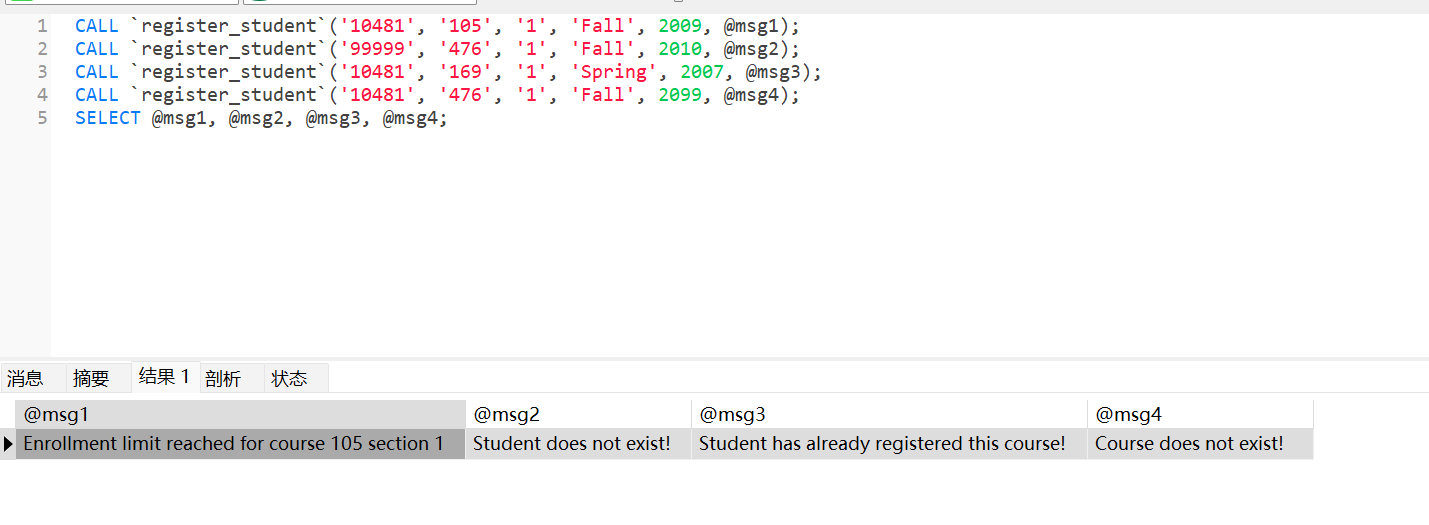
\includegraphics[width=0.9\textwidth]{img/15.png}
          \caption{测试结果}
        \end{figure}

  \item 编写一个名为 \texttt{section\_setup}的存储过程,完成下面的任务:

        \begin{itemize}
          \item 输入参数: \texttt{course\_id}
          \item 为该课程在接下来的新学期开设一个新的section;
          \item 该课程所属院系的学生如果之前没有修过该课程,则为其注册该课程;
          \item 为其它所需参数设置合理的值;
        \end{itemize}

        \begin{lstlisting}[language=sql]
DELIMITER $$
CREATE DEFINER = CURRENT_USER PROCEDURE `section_setup`(
  IN `course_id` int,
  OUT `message` varchar(100)
)
BEGIN
  #Routine body goes here...
  DECLARE `@sec_cnt` INT;
  DECLARE `@dept_name` VARCHAR(20);
  DECLARE `@sec_id` INT;
  DECLARE `@building` VARCHAR(15);
  DECLARE `@room_number` INT;
  DECLARE `@semester` VARCHAR(6);
  DECLARE `@year` INT;
  DECLARE `@cnt` INT;
  SELECT COUNT(*) INTO `@sec_cnt` FROM `course`
  WHERE `course`.`course_id` = `course_id`;
  SELECT DISTINCT `dept_name` INTO `@dept_name` FROM `course`
  WHERE `course`.`course_id` = `course_id`;
  IF (`@sec_cnt` = 0) THEN
    SET `message` = 'Course does not exist!';
  ELSE
    BEGIN
      SELECT MAX(`sec_id`) + 1 INTO `@sec_id` FROM `section`
      WHERE `section`.`course_id` = `course_id`;
      SELECT DISTINCT `building` INTO `@building` 
      FROM `department` WHERE `dept_name` = `@dept_name`;
      SELECT DISTINCT `room_number` INTO `@room_number`
      FROM `classroom` WHERE `building` = `@building`
      ORDER BY `room_number` DESC LIMIT 1;
      IF (MONTH(CURDATE()) < 2) THEN
        SET `@semester` = 'Spring';
        SET `@year` = YEAR(CURDATE());
      ELSEIF (MONTH(CURDATE()) < 8) THEN
        SET `@semester` = 'Fall';
        SET `@year` = YEAR(CURDATE());
      ELSE
        SET `@semester` = 'Spring';
        SET `@year` = YEAR(CURDATE()) + 1;
      END IF;
      SELECT COUNT(*) INTO `@cnt`
      FROM `student`
      WHERE `dept_name` = `@dept_name` AND `ID` NOT IN (
        SELECT `ID`
        FROM `takes`
        WHERE `takes`.`course_id` = `course_id`
      );
      INSERT INTO `section`
      VALUES (`course_id`, `@sec_id`, `@semester`, `@year`, `@building`, `@room_number`, 'A');
      INSERT INTO `takes`
      SELECT `ID`, `course_id`, `@sec_id`, `@semester`, `@year`, NULL
      FROM `student`
      WHERE `dept_name` = `@dept_name` AND `ID` NOT IN (
        SELECT `ID`
        FROM `takes`
        WHERE `takes`.`course_id` = `course_id`
      );
      SET `message` = CONCAT('Successfully insert ', `@cnt`, ' records.');
    END;
  END IF;
END$$
DELIMITER ;
\end{lstlisting}

        使用以下语句进行测试:

        \begin{lstlisting}[language=sql]
CALL section_setup(999, @msg1);
CALL section_setup(105, @msg2);
SELECT @msg1, @msg2;
\end{lstlisting}

结果如下:

\begin{figure}[H]
  \centering
  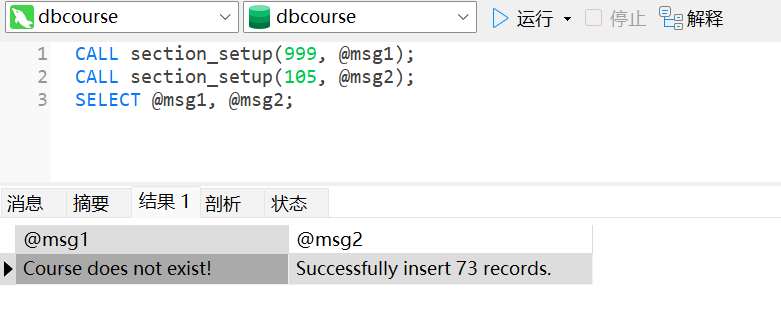
\includegraphics[width=0.8\textwidth]{img/16.png}
  \caption{测试结果}
\end{figure}

\end{enumerate}

\subsection{触发器}


\begin{enumerate}
\item 参照教材207页Figure 5.9,编写两个名为 \tt{timeslot\_check1} 和 \tt{timeslot\_check2} 的触发器;

\begin{lstlisting}[language=sql]
DELIMITER $$
CREATE TRIGGER `timeslot_check1` AFTER INSERT ON `section`
FOR EACH ROW
  IF NEW.`time_slot_id` NOT IN (
    SELECT `time_slot_id` FROM `time_slot`
  ) THEN
    SIGNAL SQLSTATE '45000' 
    SET MESSAGE_TEXT = 'The time_slot_id does not exist. The INSERT operation fails!';
  end IF$$
CREATE TRIGGER `timeslot_check2` AFTER DELETE ON `time_slot`
FOR EACH ROW
  IF OLD.`time_slot_id` NOT IN (
    SELECT `time_slot_id` FROM `time_slot`
  )
  AND OLD.`time_slot_id` IN (
    SELECT `time_slot_id` FROM `section`
  ) THEN
    SIGNAL SQLSTATE '45000' 
    SET MESSAGE_TEXT = 'The time_slot_id is referenced by some sections. The DELETE operation fails!';
  end IF$$
DELIMITER ;
\end{lstlisting}

结果如下:

\begin{figure}[H]
  \centering
  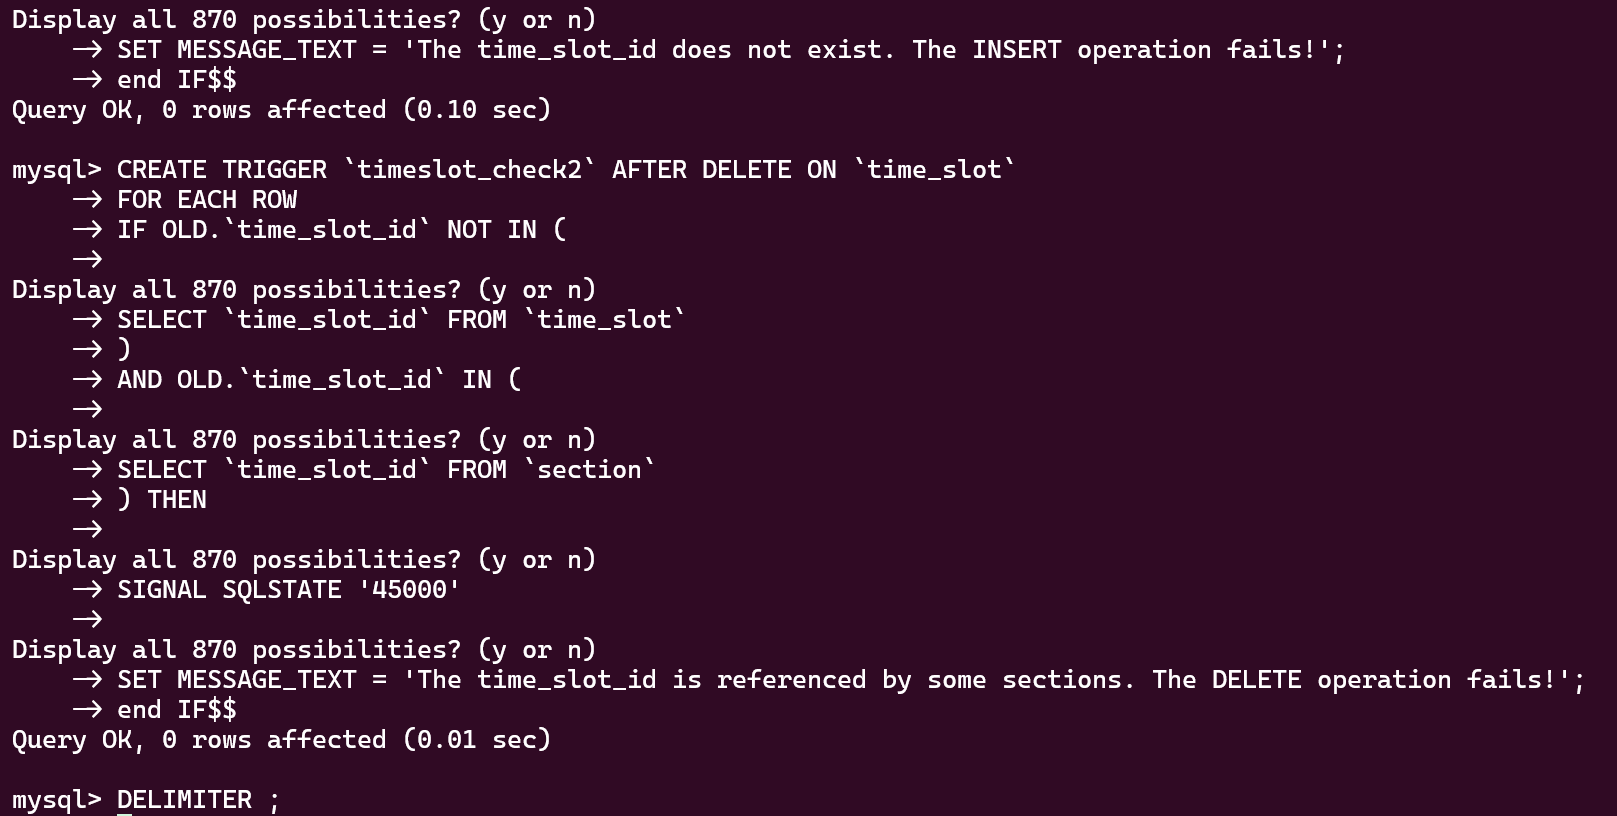
\includegraphics[width=0.7\textwidth]{img/17.png}
  \caption{创建触发器}
\end{figure}

\item 依次执行下列SQL语句并检查触发器\tt{timeslot\_check1}的执行效果;

\begin{lstlisting}[language=sql]
SELECT * FROM `time_slot` WHERE `time_slot_id` = 'Q';
INSERT INTO `section` 
VALUES('747', '1', 'Fall', 2023, 'Gates', '314', 'Q');
SELECT * FROM `section` 
WHERE `course_id` = '747' AND `sec_id` = '1' 
AND `semester`= 'Fall' AND `year` = 2023;
INSERT INTO `time_slot` VALUES('Q', 'W', 10, 0, 12, 30);
INSERT INTO `section` VALUES('747', '1', 'Fall', 2023, 'Gates', '314', 'Q');
SELECT * FROM `section` 
WHERE `course_id` = '747' AND `sec_id` = '1' 
AND `semester` = 'Fall' AND `year` = 2023;
\end{lstlisting}

结果如下:

\begin{figure}[H]
  \centering
  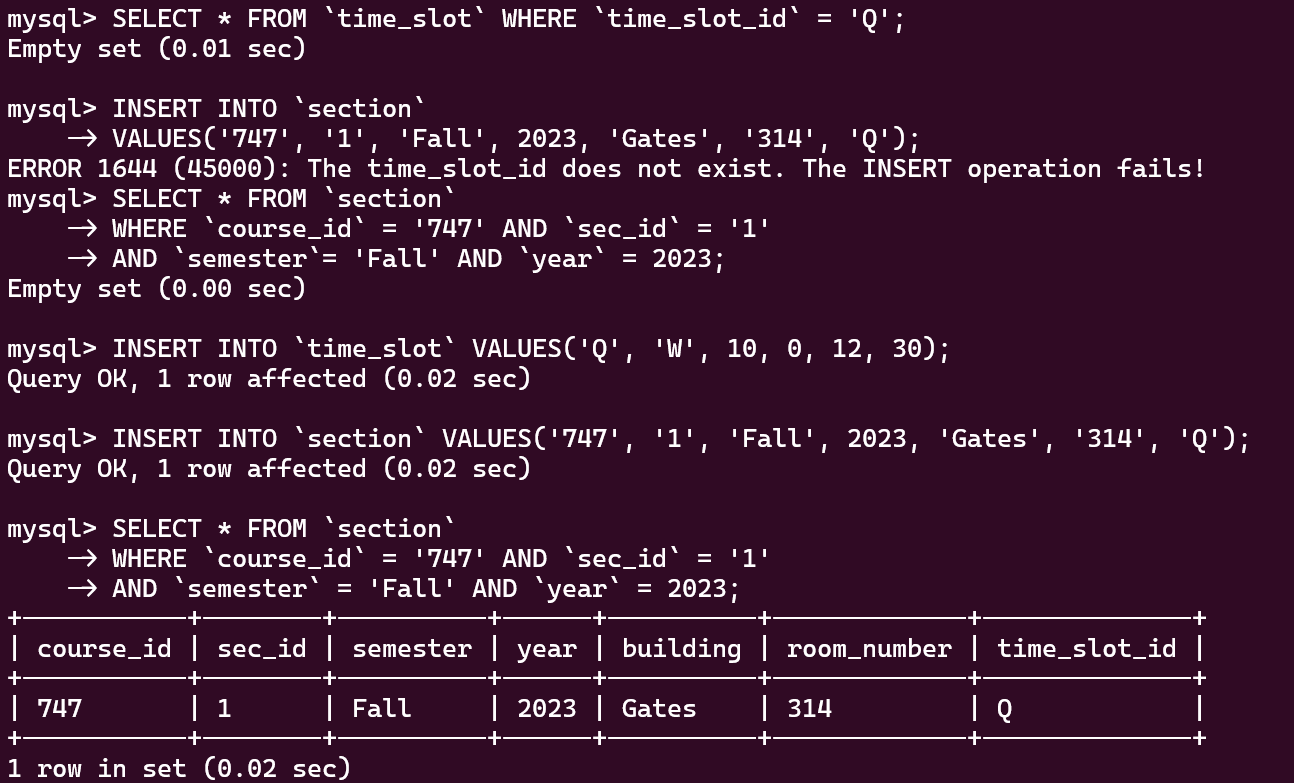
\includegraphics[width=0.9\textwidth]{img/18.png}
  \caption{测试结果}
\end{figure}

\item 依次执行下列SQL语句并检查触发器\tt{timeslot\_check2}的执行效果;

\begin{lstlisting}[language=sql]
INSERT INTO `time_slot` VALUES( 'Q', 'F', 10, 0, 12, 30);
SELECT * FROM `time_slot` WHERE `time_slot_id` = 'Q';
DELETE FROM `time_slot` WHERE `time_slot_id` = 'Q' AND `day` = 'W';
SELECT * FROM `time_slot` WHERE `time_slot_id` = 'Q';
DELETE FROM `time_slot` WHERE `time_slot_id` = 'Q' AND `day` = 'F';
SELECT * FROM `time_slot` WHERE `time_slot_id` = 'Q';
SELECT * FROM `section` WHERE `time_slot_id` = 'Q';
DELETE FROM `section` WHERE `time_slot_id` = 'Q';
DELETE FROM `time_slot` WHERE `time_slot_id` = 'Q' AND `day` = 'F';
SELECT * FROM `time_slot` WHERE `time_slot_id` = 'Q';
\end{lstlisting}

结果如下:

\begin{figure}[H]
  \centering
  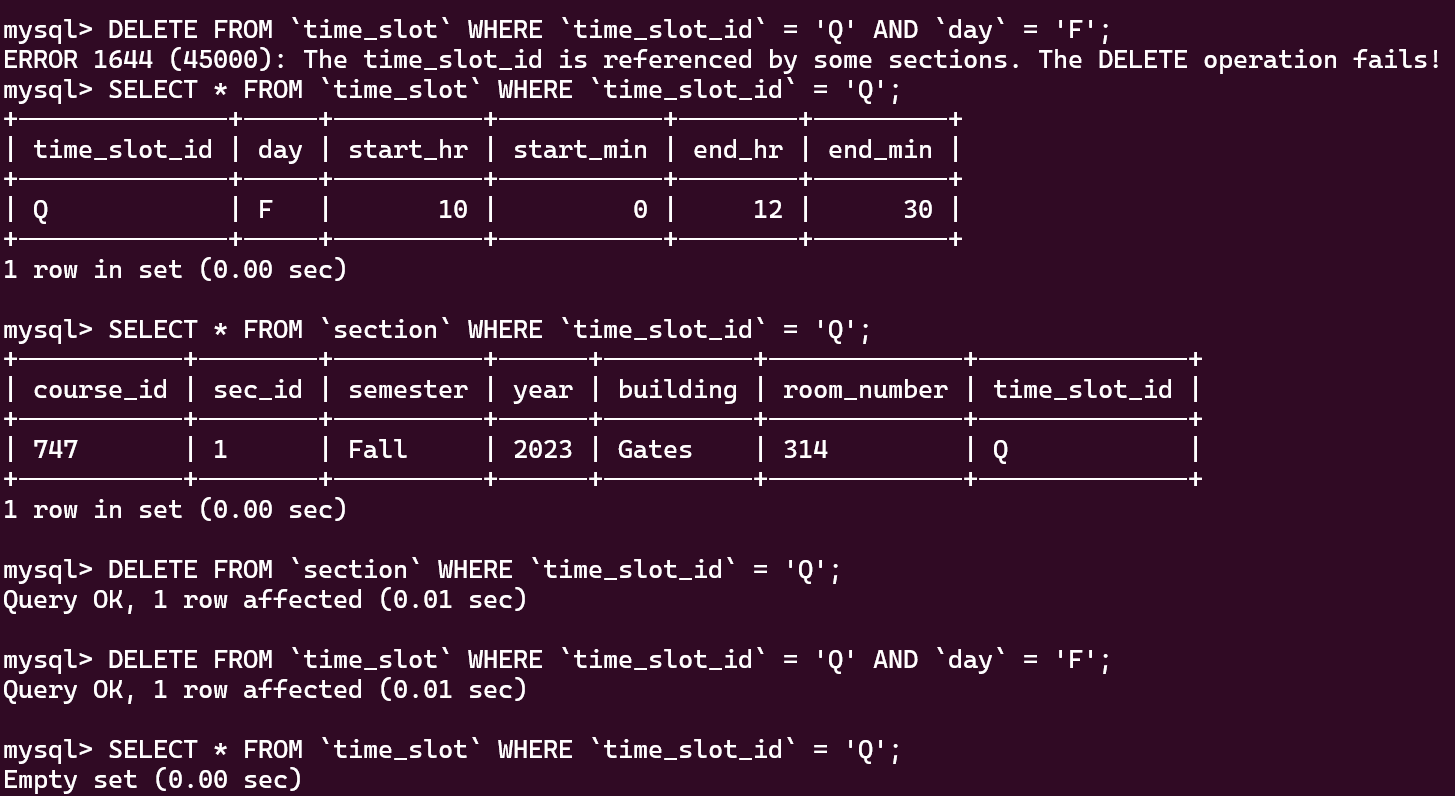
\includegraphics[width=0.9\textwidth]{img/19.png}
  \caption{测试结果}
\end{figure}

\item 执行下列SQL语句,查看并删除所创建的触发器;

\begin{lstlisting}[language=sql]
SHOW TRIGGERS \G
SELECT * FROM information_schema.triggers \G
DROP TRIGGER timeslot_check1;
DROP TRIGGER timeslot_check2;
\end{lstlisting}

结果如下:

\begin{figure}[H]
  \centering
  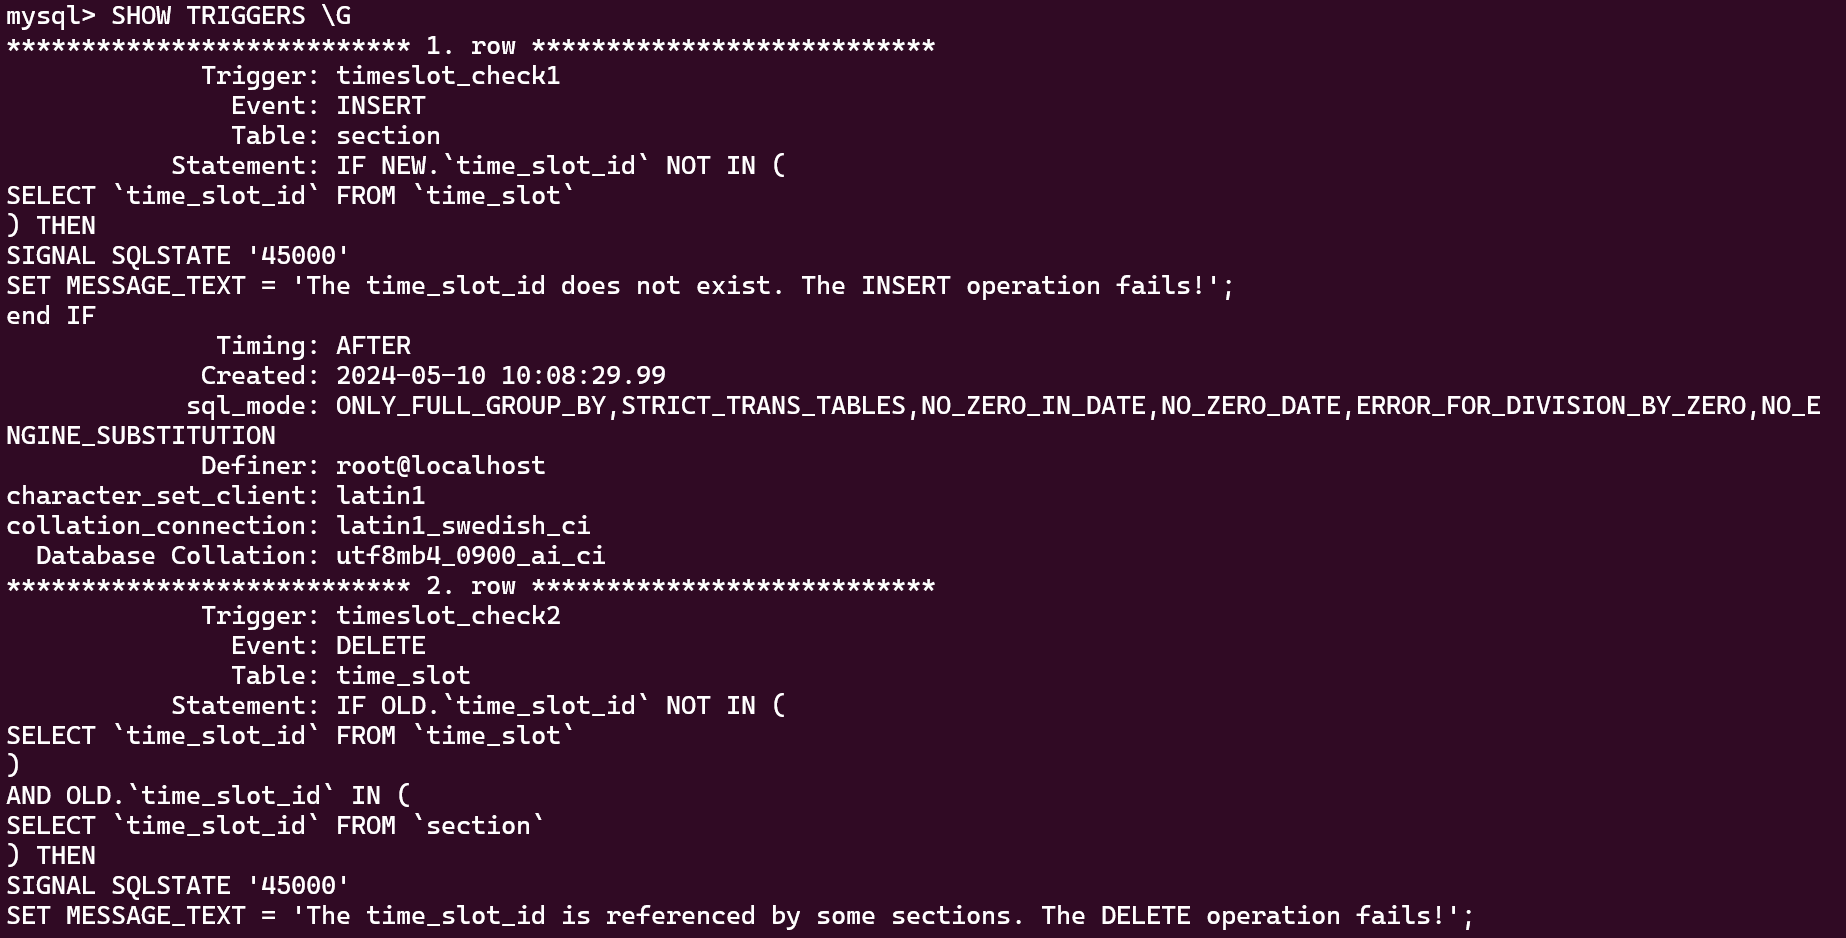
\includegraphics[width=0.9\textwidth]{img/20.png}
  \caption{查看触发器(1)}
\end{figure}

\begin{figure}[H]
  \centering
  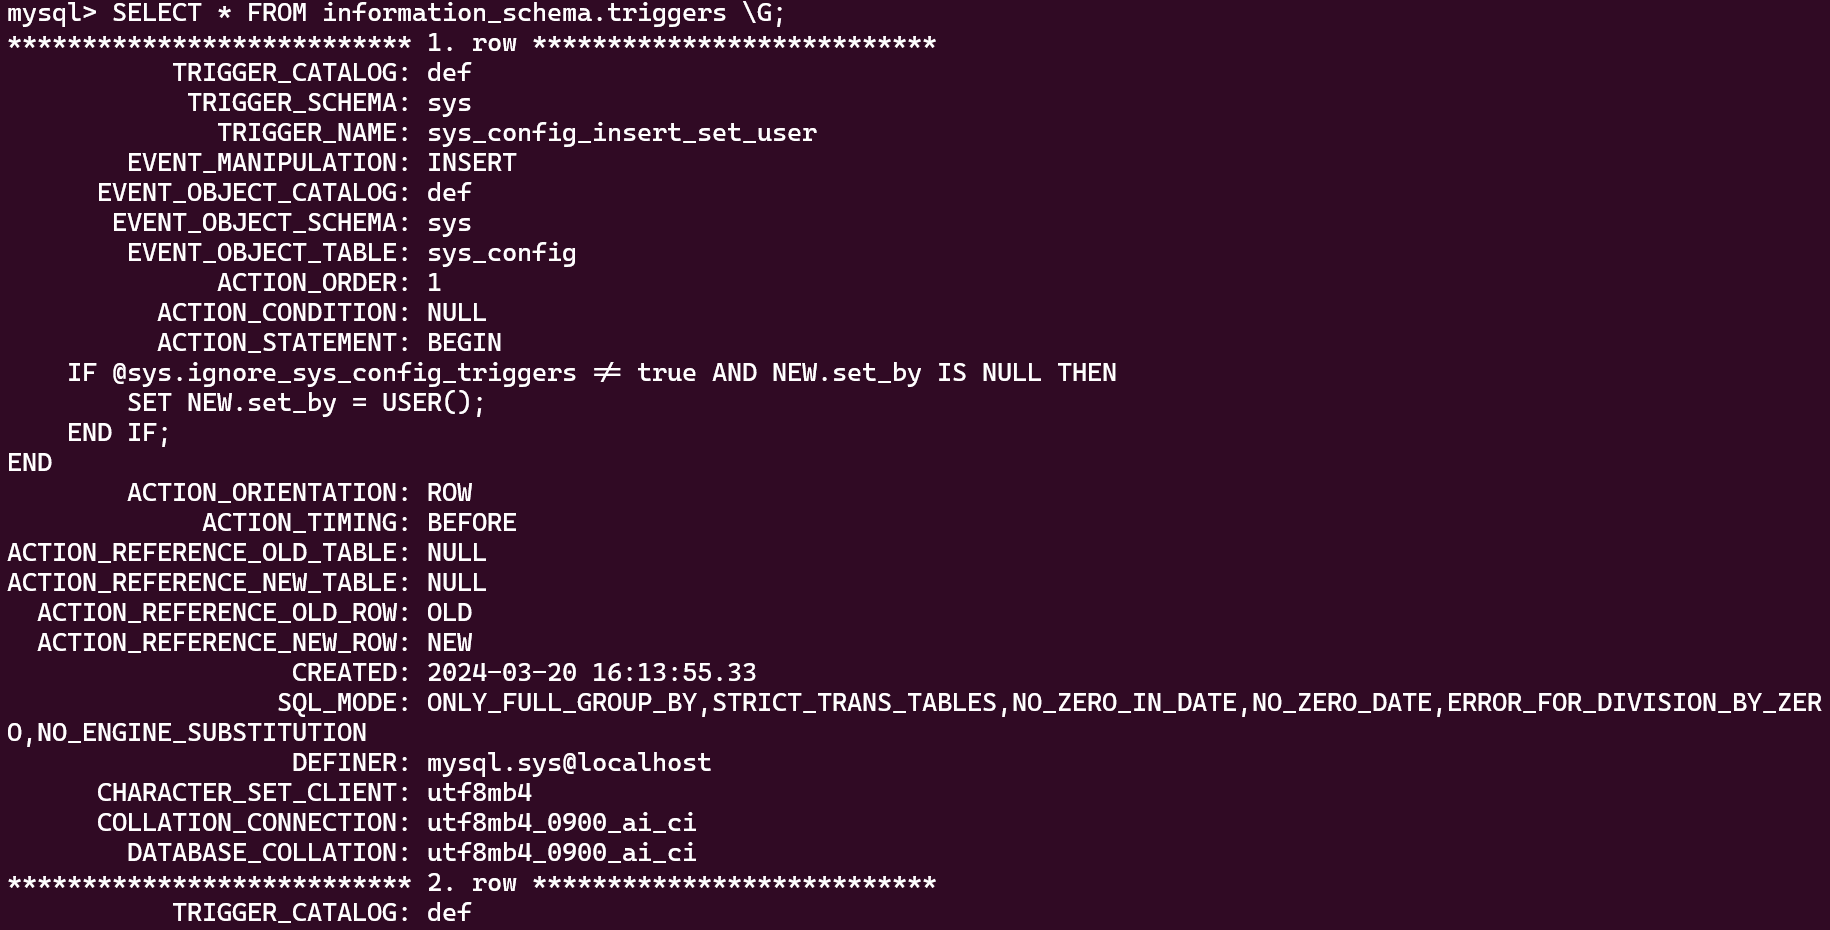
\includegraphics[width=0.9\textwidth]{img/21.png}
  \caption{查看触发器(2)}
\end{figure}

\begin{figure}[H]
  \centering
  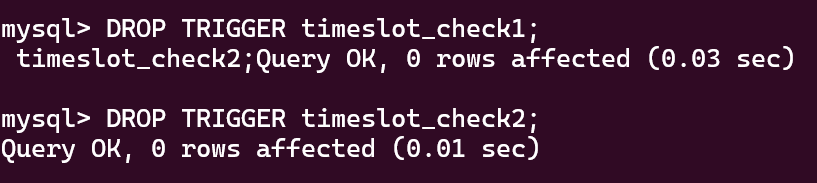
\includegraphics[width=0.9\textwidth]{img/22.png}
  \caption{删除触发器}
\end{figure}

\item 参照教材209页Figure 5.10,创建一个名为 \tt{credits\_earned} 的触发器用于维护学生所获得的学分,然后测试该触发器是否能正确执行;

\begin{lstlisting}[language=sql]
CREATE TRIGGER `credits_earned` AFTER UPDATE OF `grade` ON `takes`
FOR EACH ROW
WHEN NEW.`grade` <> 'F' AND NEW.`grade` IS NOT NULL
AND (OLD.`grade` = 'F' OR OLD.`grade` IS NULL)
BEGIN ATOMIC
    UPDATE `student`
    SET `tot_cred` = `tot_cred` + (
    SELECT `credits`
        FROM `course`
        WHERE `course`.`course_id` = NEW.`course_id`
  )
    WHERE `student`.`id` = NEW.`id`;
END;
\end{lstlisting}

\begin{figure}[H]
  \centering
  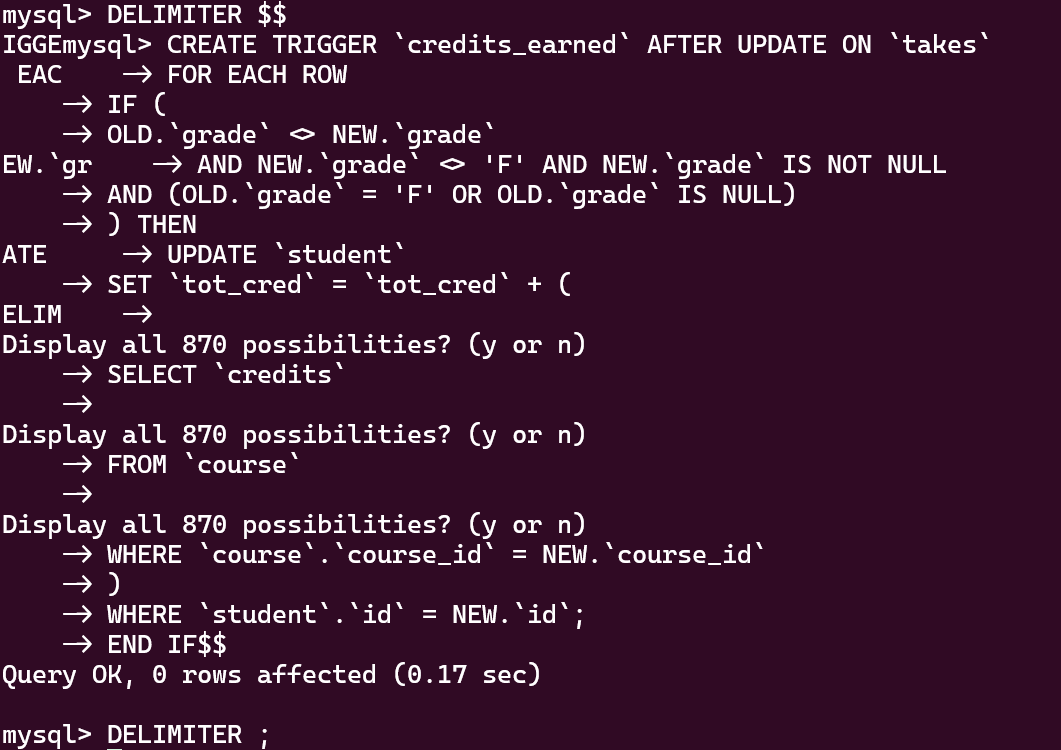
\includegraphics[width=0.52\textwidth]{img/23.png}
  \caption{创建触发器}
\end{figure}

使用以下语句进行测试:

\begin{lstlisting}[language=sql]
SELECT `tot_cred` FROM `student` WHERE `ID` = '2501';
UPDATE `takes` SET `grade` = 'A'
WHERE `ID` = '2501' AND `course_id` = '105' AND `sec_id` = '3';
SELECT `tot_cred` FROM `student` WHERE `ID` = '2501';
\end{lstlisting}

结果如下:

\begin{figure}[H]
  \centering
  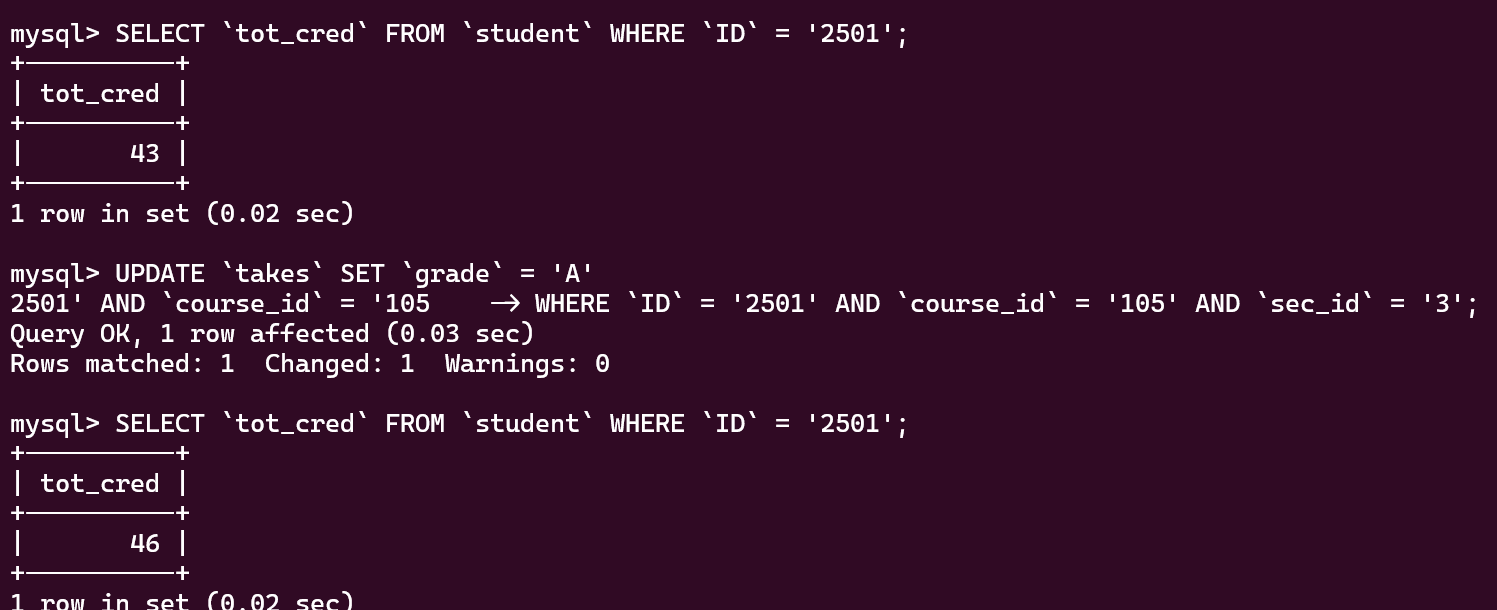
\includegraphics[width=0.9\textwidth]{img/24.png}
  \caption{测试结果}
\end{figure}

\end{enumerate}

\subsection{\tt{SQL}查询进阶}

\begin{enumerate}
\item 参照教材217页Figure 5.16,使用递归查询语句创建一个名为 \tt{rec\_prereq} 的视图,找出所有课程的直接和间接前导课程;

\begin{lstlisting}[language=sql]
CREATE VIEW `rec_prereq` AS
WITH RECURSIVE `cte` AS
(
  SELECT `course_id`, `prereq_id` FROM `prereq`
  UNION
  SELECT `cte`.`course_id`, `prereq`.`prereq_id` FROM `cte`, `prereq`
  WHERE `cte`.`prereq_id` = `prereq`.`course_id`
)
SELECT * FROM `cte';
\end{lstlisting}

\begin{figure}[H]
  \centering
  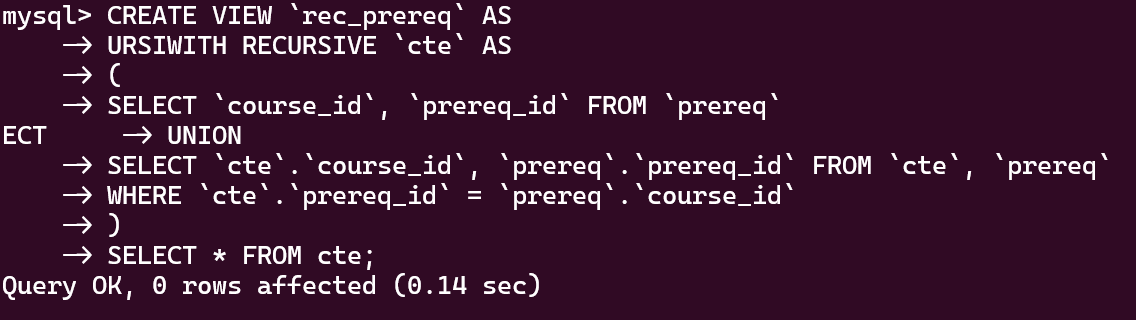
\includegraphics[width=0.9\textwidth]{img/25.png}
  \caption{创建视图}
\end{figure}

视图的内容如图所示:

\begin{figure}[H]
  \centering
  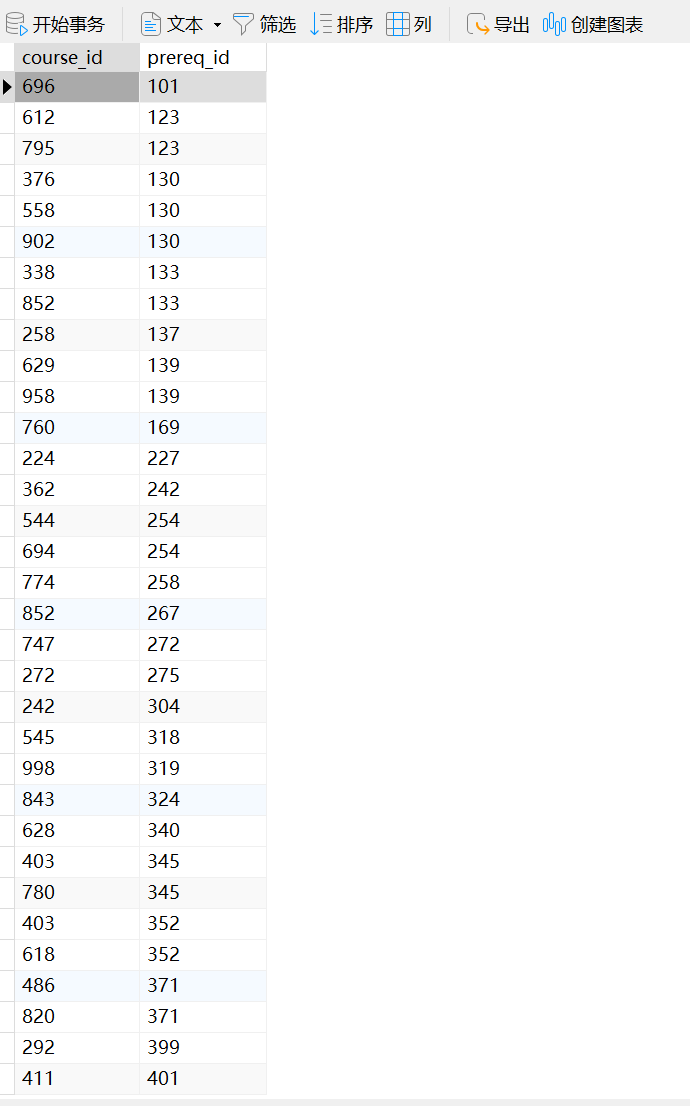
\includegraphics[width=0.45\textwidth]{img/26.png}
  \caption{视图内容}
\end{figure}

\item 执行下列SQL语句,创建一个名为 \tt{students\_gpa} 的视图;

\begin{lstlisting}[language=sql]
CREATE VIEW students_gpa AS
SELECT id, name, round(SUM(point * credits) / SUM(credits), 1) AS GPA
FROM student NATURAL LEFT OUTER JOIN
(
  SELECT id, takes.course_id, course.credits, MAX(gp) AS point
  FROM takes, grade_point, course
  WHERE TRIM(takes.grade) = grade_point.grade 
  AND takes.course_id = course.course_id
  GROUP BY id, takes.course_id, course.credits
) AS tmp
GROUP BY id, name;
\end{lstlisting}

\begin{figure}[H]
  \centering
  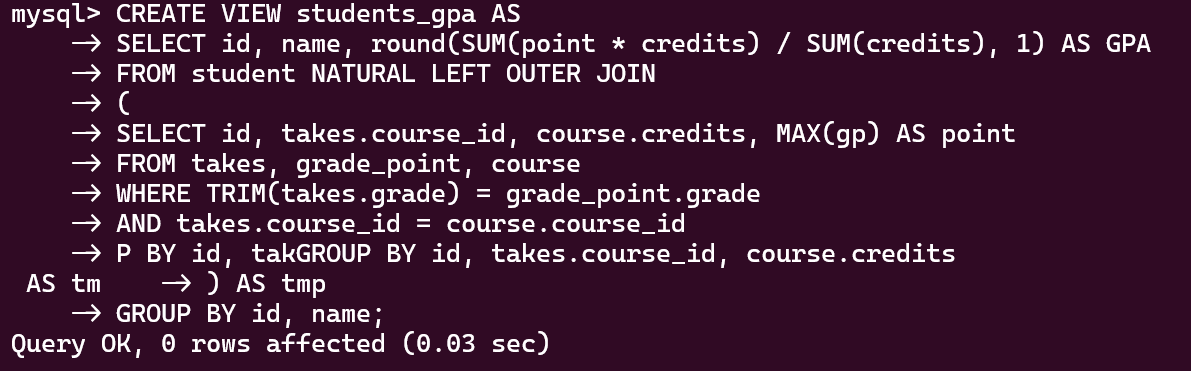
\includegraphics[width=0.9\textwidth]{img/27.png}
  \caption{创建视图}
\end{figure}

视图的内容如图所示:

\begin{figure}[H]
  \centering
  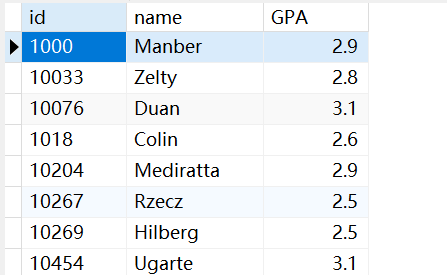
\includegraphics[width=0.45\textwidth]{img/28.png}
  \caption{视图内容}
\end{figure}

\item 编写SQL语句,按GPA的降序列出学生的ID、姓名、GPA和排名,结果按GPA排名的升序排列;

\begin{enumerate}
  \item 当名次出现并列时,下一个名次不连续;
  \begin{lstlisting}[language=sql]
SELECT `id`, `name`, `GPA`, RANK() OVER (ORDER BY `GPA` DESC) AS `rank`
FROM `students_gpa`
ORDER BY `rank`;
  \end{lstlisting}

  结果如下:

  \begin{figure}[H]
    \centering
    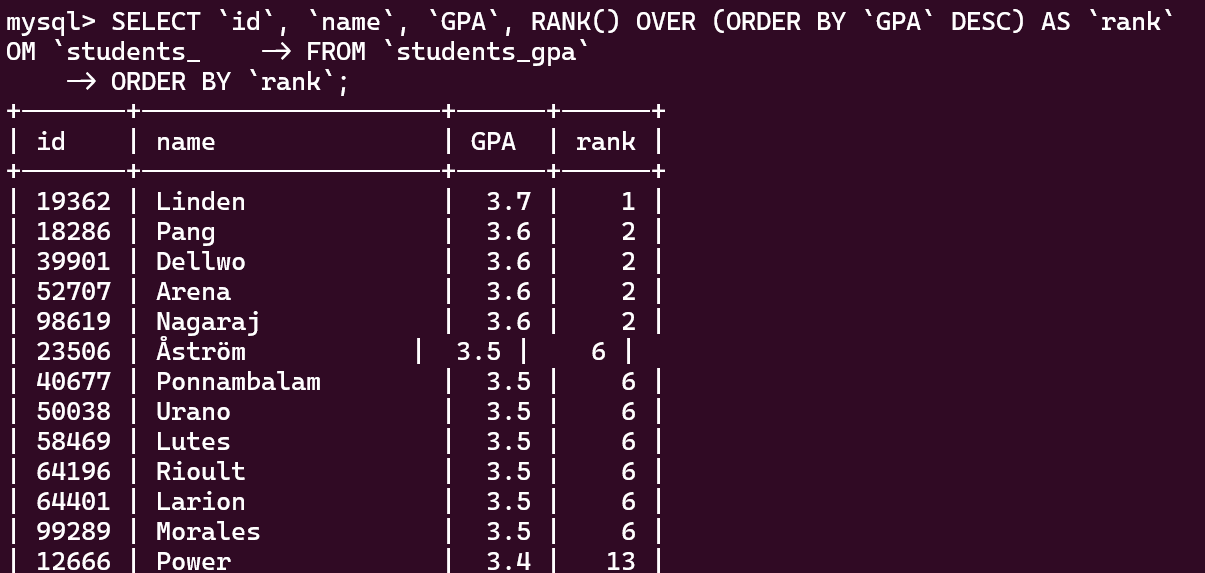
\includegraphics[width=0.65\textwidth]{img/29.png}
    \caption{查询结果}
  \end{figure}
  \item 当名次出现并列时,下一个名次连续;
  
  \begin{lstlisting}[language=sql]
SELECT `id`, `name`, `GPA`, DENSE_RANK() OVER (ORDER BY `GPA` DESC) AS `rank`
FROM `students_gpa`
ORDER BY `rank`;
  \end{lstlisting}

  结果如下:

  \begin{figure}[H]
    \centering
    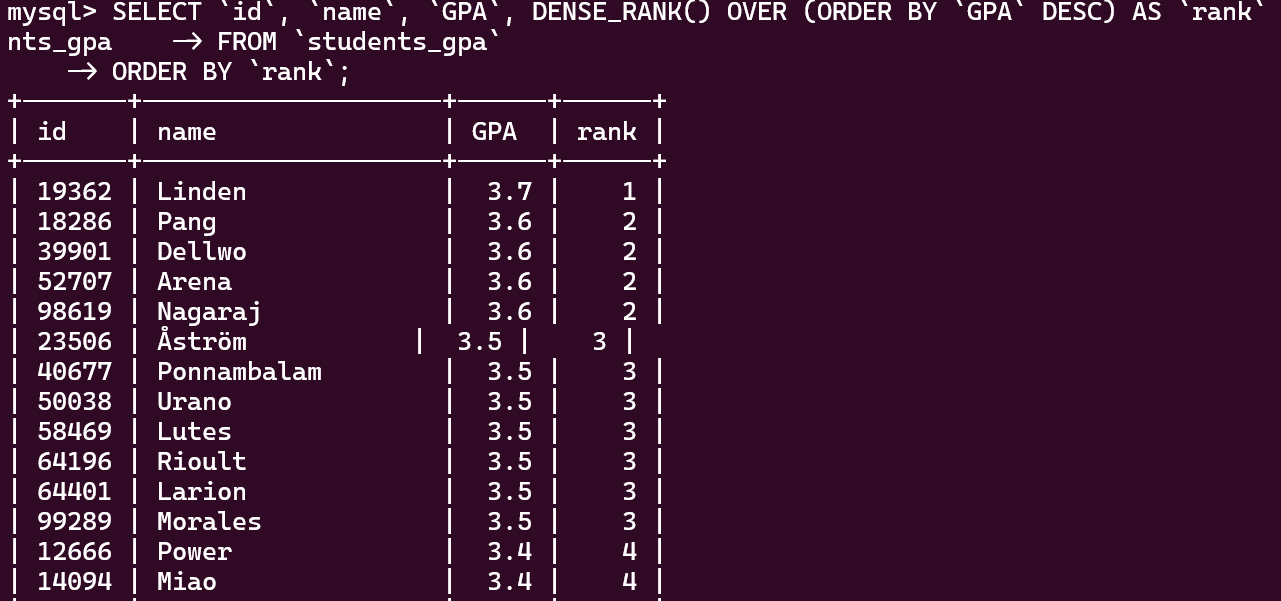
\includegraphics[width=0.65\textwidth]{img/30.png}
    \caption{查询结果}
  \end{figure}
  \item 不使用 \tt{RANK} 或 \tt{DENSE\_RANK} 函数;
  
  \begin{enumerate}
    \item 完成(a)的需求
    \begin{lstlisting}[language=sql]
SELECT `id`, `name`, `GPA`, (
  SELECT COUNT(`GPA`) + 1
  FROM `students_gpa` AS `tmp`
  WHERE `tmp`.`GPA` > `students_gpa`.`GPA`
) AS `rank`
FROM `students_gpa`
ORDER BY `rank`;
    \end{lstlisting}

    结果如下:

    \begin{figure}[H]
      \centering
      
\includegraphics[width=0.65\textwidth]{img/31.png}
      \caption{查询结果}
    \end{figure}

    \item 完成(b)的需求
    
    \begin{lstlisting}[language=sql]
SELECT `id`, `name`, `GPA`, (
  SELECT COUNT(DISTINCT `GPA`) + 1
  FROM `students_gpa` AS `tmp`
  WHERE `tmp`.`GPA` > `students_gpa`.`GPA`
) AS `rank`
FROM `students_gpa`
ORDER BY `rank`;
    \end{lstlisting}

    结果如下:

    \begin{figure}[H]
      \centering
      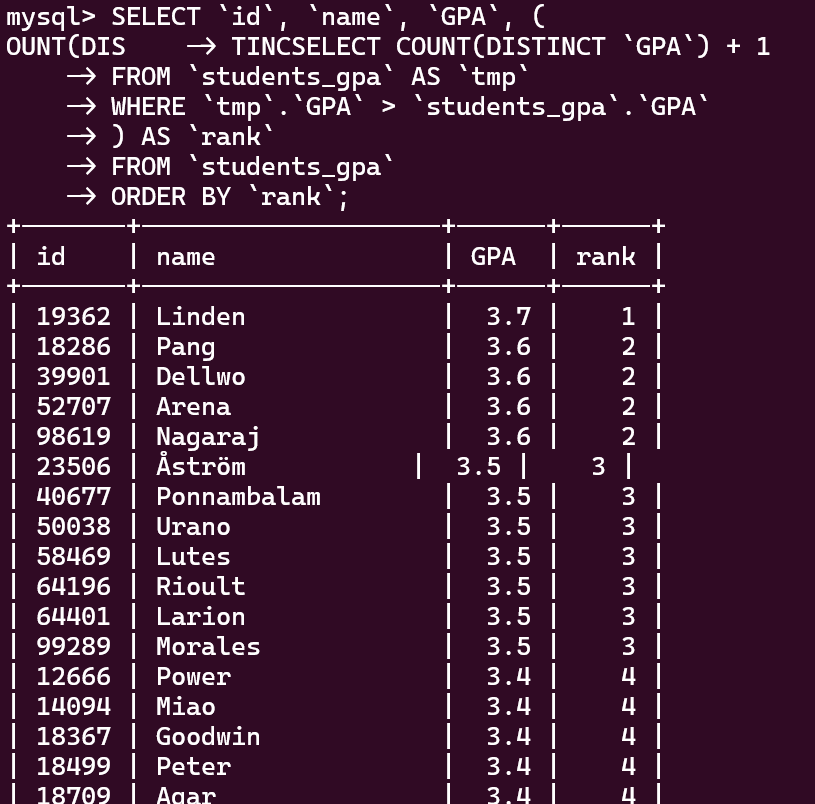
\includegraphics[width=0.65\textwidth]{img/32.png}
      \caption{查询结果}
    \end{figure}
  \end{enumerate}
\end{enumerate}

\item 执行下列SQL语句,创建一个名为 \tt{dept\_grades} 的视图;

\begin{lstlisting}[language=sql]
CREATE VIEW dept_grades AS
SELECT id, name, dept_name, 
ROUND(SUM(point * credits) / SUM(credits), 1) as GPA
FROM student NATURAL LEFT OUTER JOIN (
  SELECT id, takes.course_id, course.credits, MAX(gp) as point
  FROM takes, grade_point, course
  WHERE TRIM(takes.grade) = grade_point.grade 
  AND takes.course_id =course.course_id
  GROUP BY id, takes.course_id, course.credits
) AS tmp
GROUP BY id, name;
\end{lstlisting}

\begin{figure}[H]
  \centering
  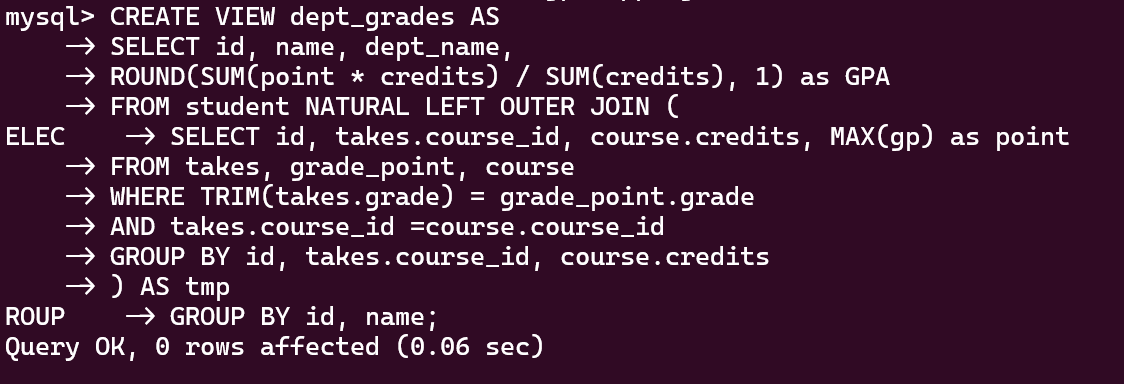
\includegraphics[width=0.9\textwidth]{img/33.png}
  \caption{创建视图}
\end{figure}

视图的内容如图所示:

\begin{figure}[H]
  \centering
  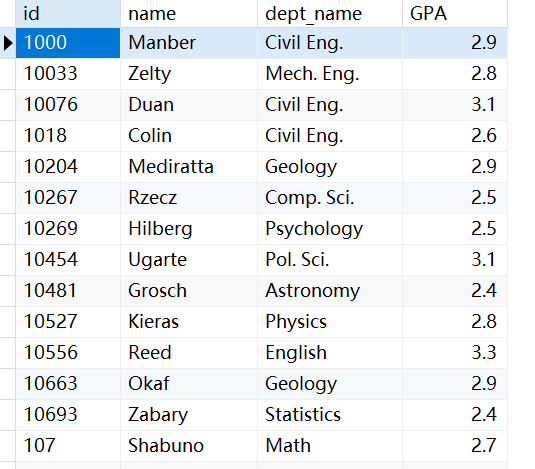
\includegraphics[width=0.45\textwidth]{img/34.png}
  \caption{视图内容}
\end{figure}

\item 编写SQL语句,按院系查询学生的GPA排名,列出学生的ID、姓名、院系、GPA和排名,结果按院
系名称和GPA排名的升序排列;

\begin{lstlisting}[language=sql]
SELECT `id`, `name`, `dept_name`, `GPA`, 
RANK() OVER (PARTITION BY `dept_name` ORDER BY `GPA` DESC) AS `rank`
FROM `dept_grades`
ORDER BY `dept_name`, `rank`;
\end{lstlisting}

结果如下:

\begin{figure}[H]
  \centering
  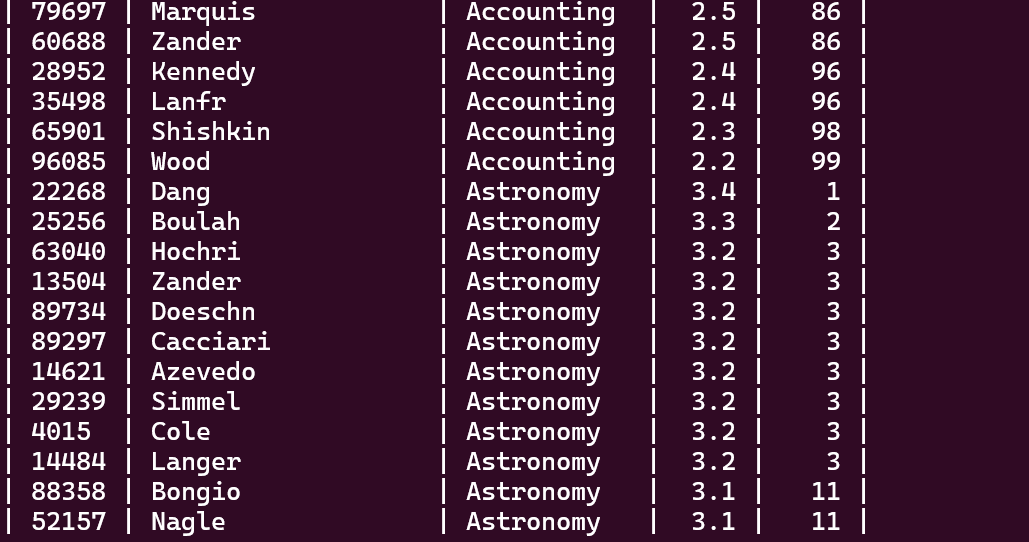
\includegraphics[width=0.9\textwidth]{img/35.png}
  \caption{查询结果}
  \end{figure}

\item 创建一个名为 \tt{tot\_credits(year, credits)} 的视图,用于统计2001年~2023年期间,每年所有学生所获得的总学分数;

\begin{lstlisting}[language=sql]
CREATE VIEW `tot_credits` (`year`, `credits`) AS
WITH `temp1` (`year`, `credits`) AS (
    SELECT `year`, SUM(`credits`) FROM `takes` NATURAL JOIN `course`
    WHERE `grade` <> 'F' OR `grade` IS NOT NULL
    GROUP BY `year`
),
`temp2` (`year`, `credits`) AS (
    SELECT 2001, 0 
  UNION SELECT 2002, 0 UNION SELECT 2003, 0 
  UNION SELECT 2004, 0 UNION SELECT 2005, 0 
  UNION SELECT 2006, 0 UNION SELECT 2007, 0 
  UNION SELECT 2008, 0 UNION SELECT 2009, 0 
  UNION SELECT 2010, 0 UNION SELECT 2011, 0 
  UNION SELECT 2012, 0 UNION SELECT 2013, 0 
  UNION SELECT 2014, 0 UNION SELECT 2015, 0 
  UNION SELECT 2016, 0 UNION SELECT 2017, 0 
  UNION SELECT 2018, 0 UNION SELECT 2019, 0 
  UNION SELECT 2020, 0 UNION SELECT 2021, 0 
  UNION SELECT 2022, 0 UNION SELECT 2023, 0
)
SELECT * FROM `temp1` UNION
SELECT * FROM `temp2` WHERE `year` NOT IN (SELECT `year` FROM `temp1`);
\end{lstlisting}

\begin{figure}[H]
  \centering
  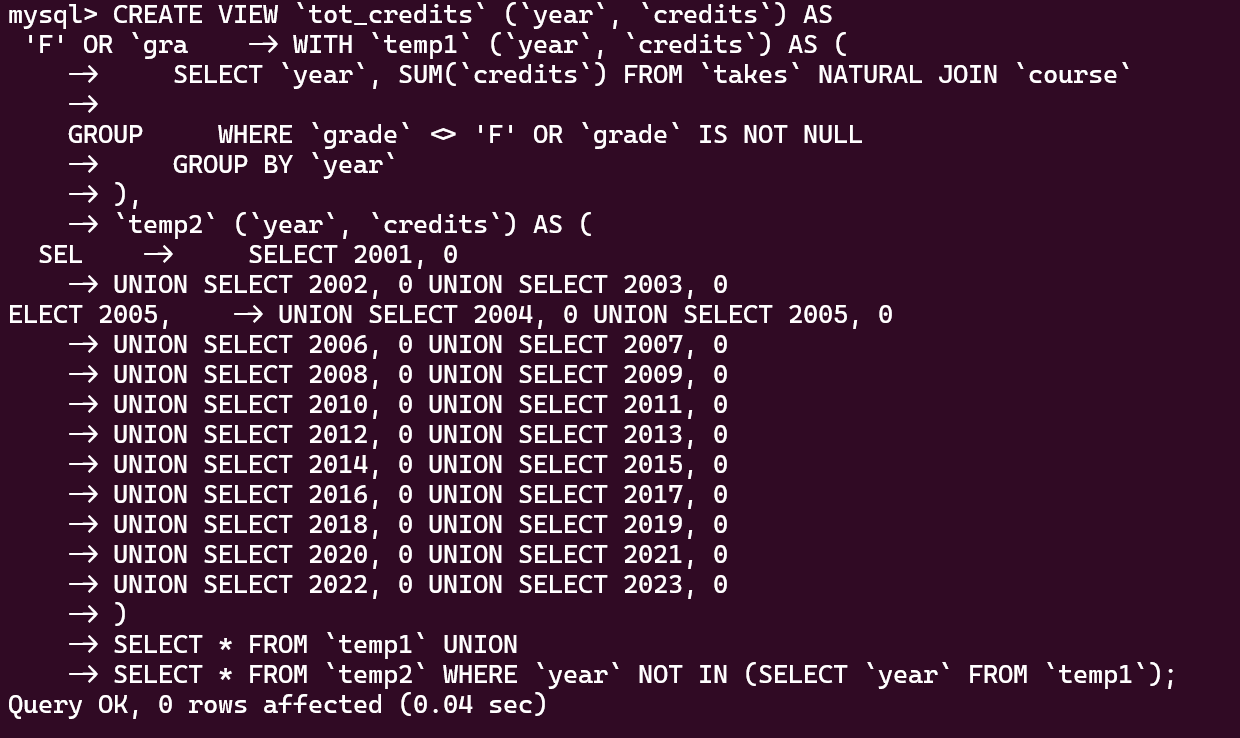
\includegraphics[width=0.9\textwidth]{img/36.png}
  \caption{创建视图}
\end{figure}

视图的内容如图所示:

\begin{figure}[H]
  \centering
  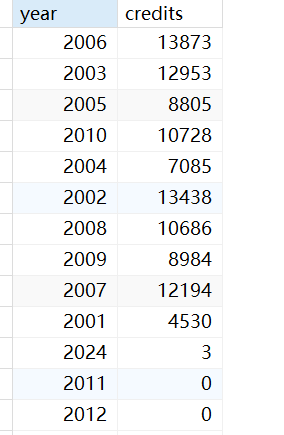
\includegraphics[width=0.25\textwidth]{img/37.png}
  \caption{视图内容}
\end{figure}

\item 编写SQL语句,使用窗口函数查询不同条件下每年所有学生所获得的总学分数的平均值;

\begin{enumerate}
  \item 前三年至今总学分数的平均值;
  
  \begin{lstlisting}[language=sql]
SELECT `year`, 
AVG(`credits`) OVER (
  ORDER BY `year` ROWS BETWEEN 3 PRECEDING AND CURRENT ROW
) AS `avg_credits`
FROM `tot_credits`;
  \end{lstlisting}

  结果如下:

  \begin{figure}[H]
    \centering
    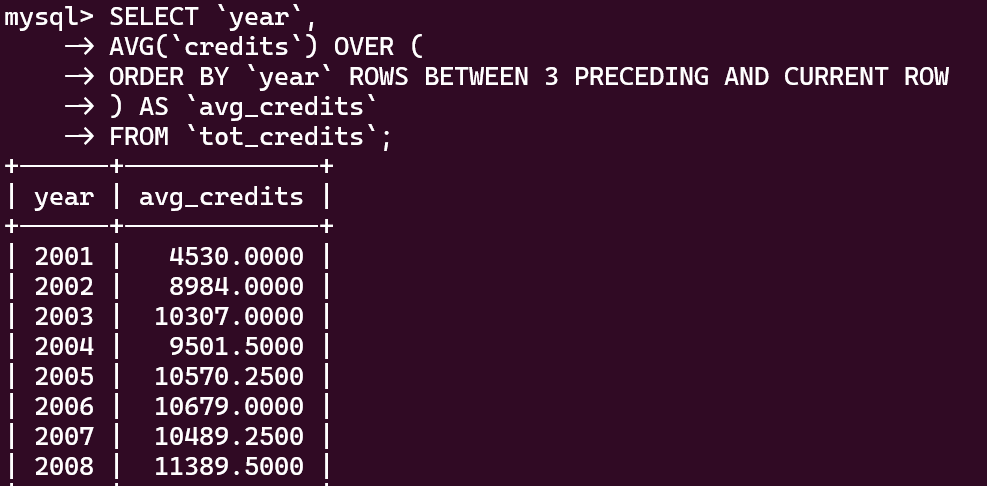
\includegraphics[width=0.9\textwidth]{img/38.png}
    \caption{查询结果}
  \end{figure}
  \item 从2001年起至今总学分数的平均值;
\begin{lstlisting}[language=sql]
SELECT `year`,
AVG(`credits`) OVER (
  ORDER BY `year` ROWS BETWEEN UNBOUNDED PRECEDING AND CURRENT ROW
) AS `avg_credits`
FROM `tot_credits`;
\end{lstlisting}

结果如下:

\begin{figure}[H]
  \centering
  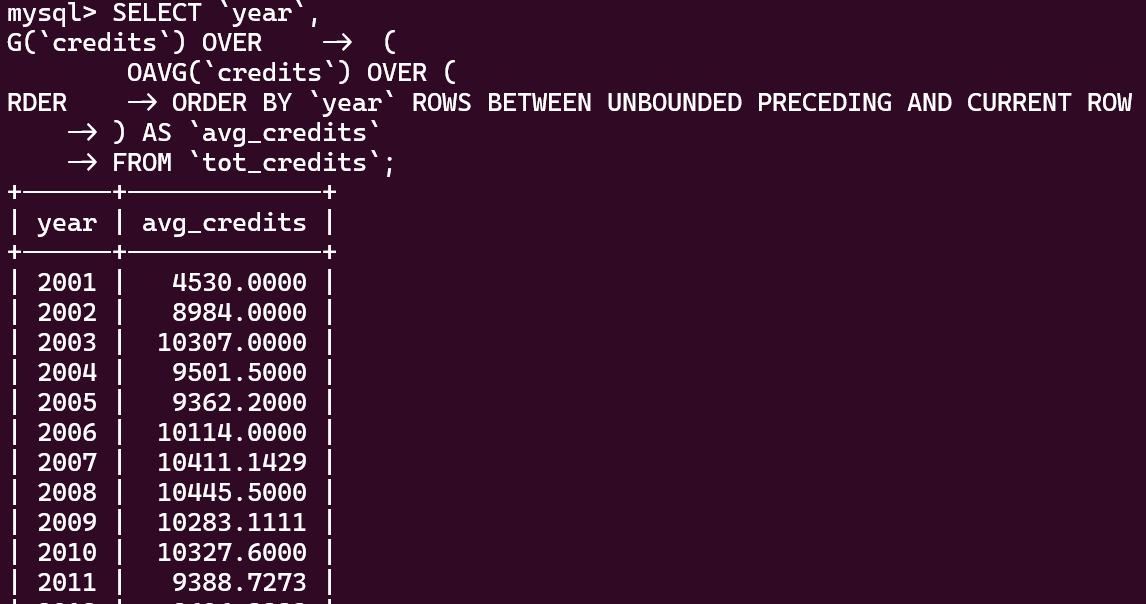
\includegraphics[width=0.7\textwidth]{img/39.png}
  \caption{查询结果}
\end{figure}
  \item 前后五年总学分数的平均值;
  
  \begin{lstlisting}[language=sql]
  SELECT `year`,
  AVG(`credits`) OVER (
    ORDER BY `year` ROWS BETWEEN 5 PRECEDING AND 5 FOLLOWING
  ) AS `avg_credits`
  FROM `tot_credits`;
  \end{lstlisting}

  结果如下:

  \begin{figure}[H]
    \centering
    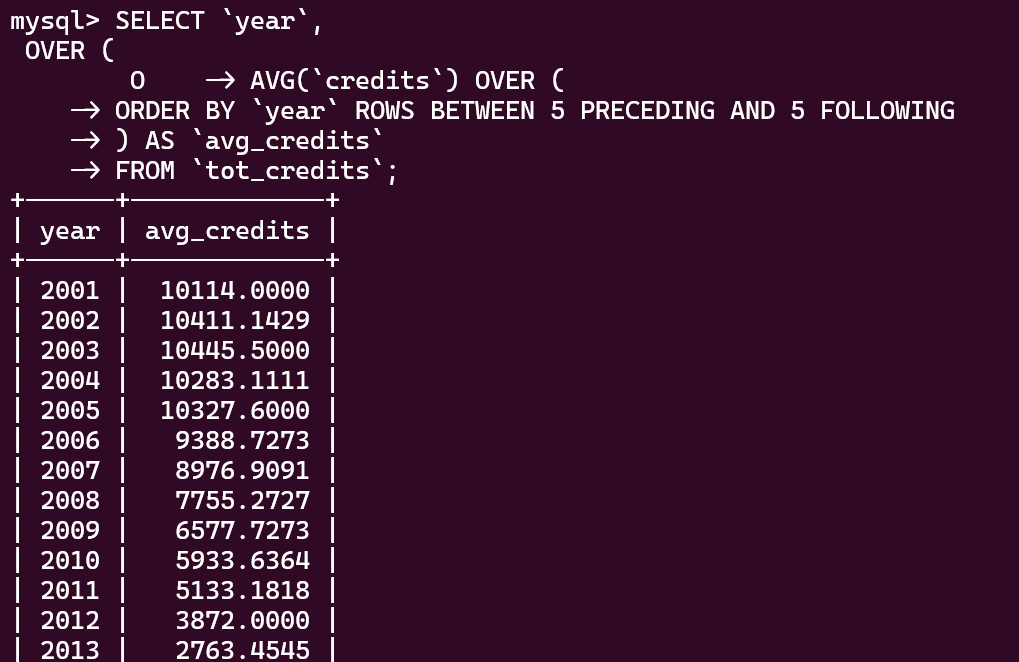
\includegraphics[width=0.65\textwidth]{img/40.png}
    \caption{查询结果}
  \end{figure}
\end{enumerate}

\item 创建一个名为 \tt{student\_tot\_credits(id, year, credits)} 的视图,用于统计每个学生每年所获得的总学分;

\begin{lstlisting}[language=sql]
CREATE VIEW `student_tot_credits` (`id`, `year`, `credits`) AS
WITH `temp1` (`id`, `year`, `credits`) AS (
  SELECT `id`, `year`, SUM(`credits`) FROM `takes` NATURAL JOIN `course`
  WHERE `grade` <> 'F' OR `grade` IS NOT NULL
  GROUP BY `id`, `year`
),
`temp2` (`id`, `year`, `credits`) AS (
  SELECT 0, 2001, 0 
  UNION SELECT 0, 2002, 0 UNION SELECT 0, 2003, 0 
  UNION SELECT 0, 2004, 0 UNION SELECT 0, 2005, 0 
  UNION SELECT 0, 2006, 0 UNION SELECT 0, 2007, 0 
  UNION SELECT 0, 2008, 0 UNION SELECT 0, 2009, 0 
  UNION SELECT 0, 2010, 0 UNION SELECT 0, 2011, 0 
  UNION SELECT 0, 2012, 0 UNION SELECT 0, 2013, 0 
  UNION SELECT 0, 2014, 0 UNION SELECT 0, 2015, 0 
  UNION SELECT 0, 2016, 0 UNION SELECT 0, 2017, 0 
  UNION SELECT 0, 2018, 0 UNION SELECT 0, 2019, 0 
  UNION SELECT 0, 2020, 0 UNION SELECT 0, 2021, 0 
  UNION SELECT 0, 2022, 0 UNION SELECT 0, 2023, 0
  UNION SELECT 0, 2024, 0
)
SELECT * FROM `temp1` UNION
SELECT * FROM `temp2` WHERE `year` NOT IN (SELECT `year` FROM `temp1`)
AND `id` <> 0;
\end{lstlisting}

\begin{figure}[H]
  \centering
  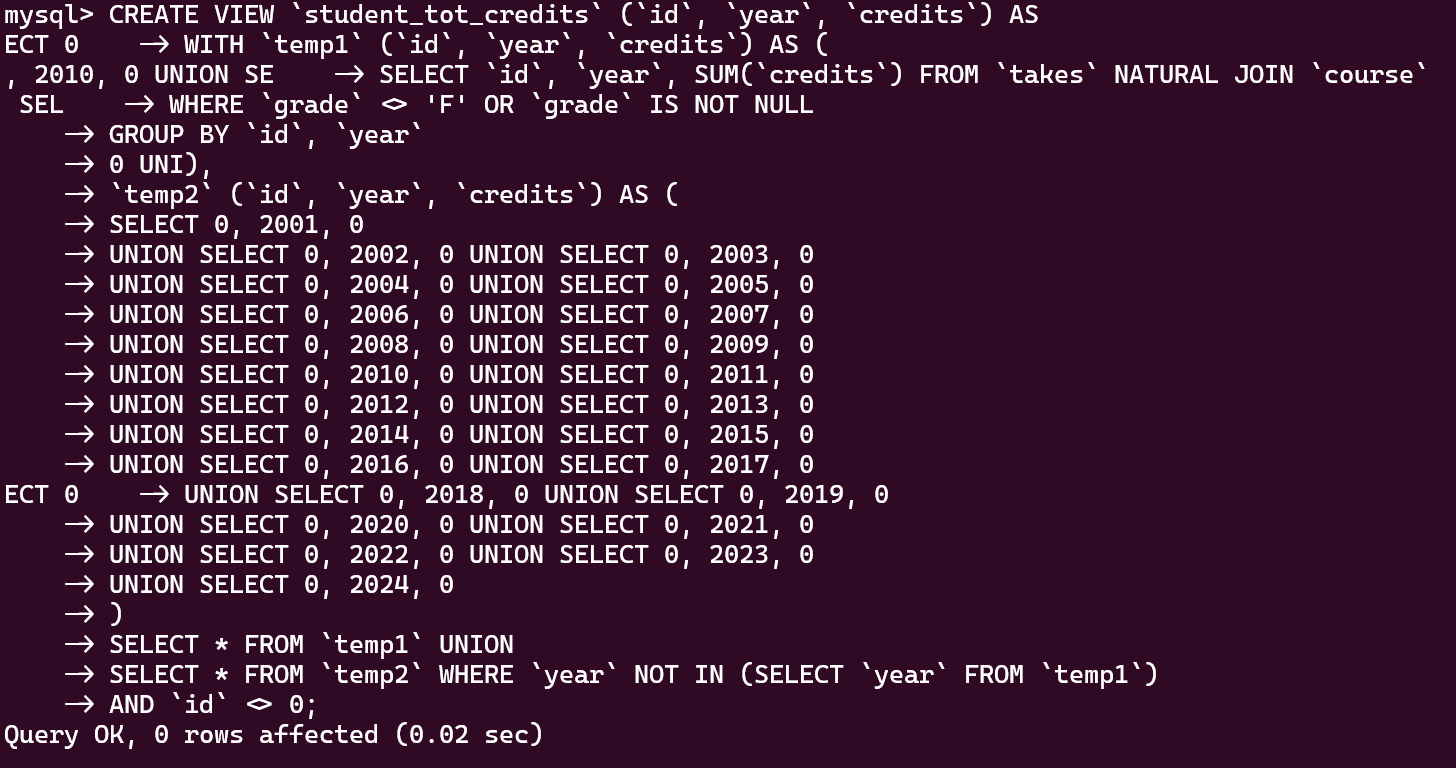
\includegraphics[width=0.69\textwidth]{img/41.png}
  \caption{创建视图}
\end{figure}

视图的内容如图所示:

\begin{figure}[H]
  \centering
  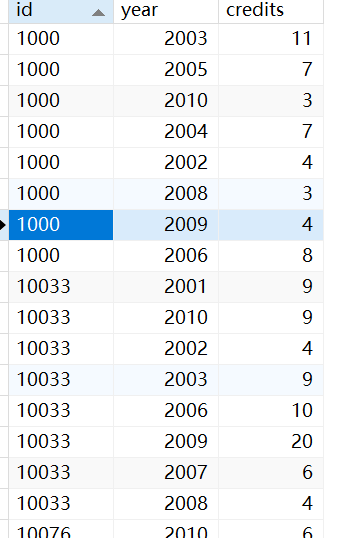
\includegraphics[width=0.3\textwidth]{img/42.png}
  \caption{视图内容}
\end{figure}

\item 编写SQL语句查询每个学生连续三年所获得的平均学分数;

\begin{lstlisting}[language=sql]
SELECT `id`, `year`,
AVG(`credits`) OVER (
  PARTITION BY `id` ORDER BY `year` ROWS BETWEEN 2 PRECEDING AND CURRENT ROW
) AS `avg_credits`
FROM `student_tot_credits`;
\end{lstlisting}

结果如下:

\begin{figure}[H]
  \centering
  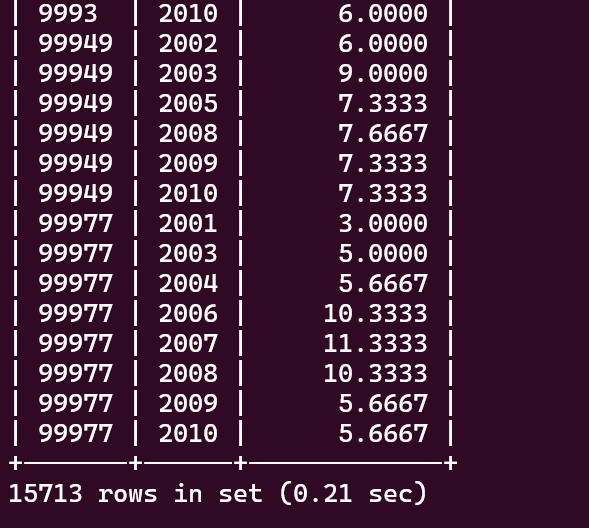
\includegraphics[width=0.5\textwidth]{img/43.png}
  \caption{查询结果}
\end{figure}

\end{enumerate}

\section{存在的问题及解决方案}

\begin{enumerate}
  \item 在使用 \texttt{INSERT INTO SELECT ...} 语句时频繁报错,原因是 \texttt{SELECT} 的表不能是使用 \texttt{WITH ...} 语句创建的表。解决方案:在此类情况时避免使用 \texttt{WITH ...} 语句;
  \item 创建存储过程时自定义变量与列名重合导致错误。解决方案:在创建存储过程时避免使用与列名重合的自定义变量名。
\end{enumerate}


\section{实验小结}

本次实验主要学习了MySQL数据库的高级应用,包括存储过程、触发器、视图和窗口函数等。通过实验,我学会了如何创建存储过程、触发器和视图,以及如何使用窗口函数进行高级查询。这些内容对于提高数据库的查询效率和数据处理能力非常有帮助。同时,实验中还遇到了一些问题,如自定义变量与列名重合导致错误等,通过查阅文档和调试代码,我成功解决了这些问题。总的来说,本次实验收获颇丰,对MySQL数据库的高级应用有了更深入的了解。

\end{document}